% !TEX program = pdflatex
\documentclass[12pt, a4paper]{article}

% --- IMF WORKING PAPER PREAMBLE ---
\usepackage[utf8]{inputenc}
\usepackage[T1]{fontenc}
\usepackage[a4paper, top=2.5cm, bottom=2.5cm, left=2cm, right=2cm]{geometry}
\usepackage[english]{babel}
\usepackage[scaled]{helvet}
\usepackage{mathptmx}
\usepackage{amsmath, amssymb, amsthm}
\usepackage{bm}
\usepackage{setspace}
\usepackage{natbib}
\usepackage{booktabs}
\usepackage{tabularx}
\usepackage{graphicx}
\usepackage{caption}
\usepackage{float}
\renewcommand{\topfraction}{0.9}
\renewcommand{\bottomfraction}{0.8}
\renewcommand{\textfraction}{0.07}
\renewcommand{\floatpagefraction}{0.75}
\setcounter{topnumber}{4}
\setcounter{totalnumber}{10}
\usepackage{tikz}
\usepackage{xcolor}
\usepackage{tocloft}
\cftsetindents{section}{0em}{3.5em}
\cftsetindents{subsection}{3.5em}{3.5em}
\usepackage[colorlinks=true, linkcolor=darkgray, citecolor=darkgray, urlcolor=darkgray, linktoc=all]{hyperref}
\newcolumntype{Y}{>{\centering\arraybackslash}X}
\renewcommand{\thesection}{\Roman{section}.}
\renewcommand{\thesubsection}{\Alph{subsection}.}
\newcommand\blfootnote[1]{%
  \begingroup
  \renewcommand\thefootnote{}\footnote{#1}%
  \addtocounter{footnote}{-1}%
  \endgroup
}
\newtheorem{proposition}{Proposition}
\newtheorem{corollary}{Corollary}
\setlength{\emergencystretch}{1.5em}
\newcommand{\PaperTitle}{The Consumer of Last Resort: External Demand and Crisis Recovery}

\begin{document}

% ==========================================
% IMF WORKING PAPER COVER & METADATA PAGES
% ==========================================
\begingroup
\singlespacing
\sffamily
\thispagestyle{empty}

% --- PAGE 1: COVER PAGE ---
\begin{tikzpicture}[remember picture, overlay]
    \fill[gray!80] ([xshift=-2.5cm]current page.north east) rectangle (current page.south east);
    \node[rotate=-90, text=white, font=\fontsize{36}{40}\selectfont\sffamily\bfseries, anchor=center]
        at ([xshift=-1.25cm]current page.east) {W O R K I N G \ \ P A P E R};
\end{tikzpicture}

\vspace*{1cm}
{\color{gray} \Large INTERNATIONAL MONETARY FUND \par}

\vspace{3cm}
\begin{minipage}{0.75\textwidth}
{\fontsize{26}{32}\selectfont \bfseries \PaperTitle \par}

\vspace{2cm}
{\Large Yurii Sholomytskyi \par}

\vspace{1.5cm}
{\large WP/\colorbox{yellow}{26/XX} \par}
\end{minipage}

\vfill
\begin{minipage}{0.65\textwidth}
\scriptsize \color{gray}
\noindent \fbox{%
    \parbox{\dimexpr\textwidth-2\fboxsep-2\fboxrule}{%
        IMF Working Papers describe research in progress by the author(s) and are published to elicit comments and to encourage debate. The views expressed in IMF Working Papers are those of the author(s) and do not necessarily represent the views of the IMF, its Executive Board, or IMF management.
    }%
}

\vspace{1.5cm}
{\fontsize{40}{48}\selectfont \bfseries 2026 \par}
\vspace{0.2cm}
{\Large August \par}
\end{minipage}

\clearpage
\setcounter{page}{1}
\rmfamily

% --- PAGE 2: METADATA & ABSTRACT ---
\vspace*{1cm}
\begin{center}
    {\small \copyright 2026 International Monetary Fund \hfill WP/\colorbox{yellow}{26/XX} \par}

    \vspace{1.5cm}
    {\bfseries IMF Working Paper \par}
    Institute for Capacity Development \par

    \vspace{1cm}
    {\bfseries \PaperTitle \par}

    \vspace{0.5cm}
    Prepared by Yurii Sholomytskyi \par

    \vspace{0.5cm}
    Authorized for distribution by Ali Alichi \par
    August 2026 \par
\end{center}

\vspace{1cm}
\noindent\fbox{%
    \parbox{\dimexpr\textwidth-2\fboxsep-2\fboxrule}{%
        \scriptsize \textbf{IMF Working Papers describe research in progress by the author(s) and are published to elicit comments and to encourage debate.} The views expressed in IMF Working Papers are those of the author(s) and do not necessarily represent the views of the IMF, its Executive Board, or IMF management.
    }%
}

\vspace{1cm}
\noindent \textbf{ABSTRACT:} External demand is closely associated with recovery from downturns in emerging and developing economies. We identify 263 downturns in 34 economies from monthly activity indicators and measure foreign demand by combining export shares observed before each downturn with subsequent growth in trading-partner economies. Recoveries are generally faster and involve smaller output losses when established export markets in advanced economies continue to expand. Overall trade openness carries no comparable association. The United States accounts for most of the baseline result: a one-percentage-point increase in the US demand contribution, calculated as the pre-downturn US export share multiplied by US growth, is associated with a reduction of about six months in the duration of a full negative cycle, after controlling for downturn depth and the presence of an IMF-supported arrangement. Broader measures of recovery continue to show a role for demand from advanced economies, although the relative importance of the United States varies with the dating of the recovery. A stylized core-periphery model shows how expansions of similar size in a core economy can have different effects abroad when their import content differs. Taken together, the findings show that recovery depends on growth in the markets that purchase a country’s exports and on the demand for imports generated by that growth.
\vspace{0.3cm}
\begin{table}[H]
    \small
    \begin{tabularx}{\textwidth}{@{}lX@{}}
        \toprule
        JEL Classification Numbers: & F14, F44, E32, F42 \\ \midrule
        Keywords: & crisis recovery, external demand, regional hubs, shift-share, output gap, trade linkages, composition of growth, global spillovers \\ \midrule
        Author's E-Mail Address: & ysholomytskyi@imf.org \\ \bottomrule
    \end{tabularx}
\end{table}

\clearpage

% --- PAGE 3: INNER TITLE PAGE ---
\vspace*{2cm}
{\color{gray!80} \Large \sffamily \textbf{WORKING PAPERS} \par}

\vspace{2cm}
{\huge \bfseries \sffamily \PaperTitle \par}

\vspace{2cm}
{\large \sffamily Prepared by Yurii Sholomytskyi \par}

\vfill
{\scriptsize \color{gray} INTERNATIONAL MONETARY FUND \par}

\clearpage
\endgroup

% --- TABLE OF CONTENTS ---
\sffamily
\tableofcontents
\clearpage
\rmfamily

\section*{Abbreviations}
\addcontentsline{toc}{section}{Abbreviations}
\vspace{0.3cm}
\noindent\renewcommand{\arraystretch}{1.25}\begin{tabular}{@{}l@{\hskip 2.5em}l@{}}
AI & Artificial intelligence \\
EU & European Union \\
GDP & Gross domestic product \\
HP & Hodrick--Prescott (filter) \\
IMF & International Monetary Fund \\
IMTS & International Trade in Goods Statistics \\
LP & Local projections \\
MONA & Monitoring of Fund Arrangements \\
UNCTAD & UN Conference on Trade and Development \\
US & United States \\
WDI & World Development Indicators \\
WEO & World Economic Outlook \\
WTO & World Trade Organization \\
X-13 & X-13ARIMA-SEATS seasonal adjustment \\
\end{tabular}

\clearpage
\onehalfspacing

\section{Introduction} \blfootnote{\emph{Disclosure of AI use.} An AI large language model was used to develop the code for the paper's data pipeline and figures and to assist with language and grammar editing. The author is responsible for the analysis, results, conclusions, and any remaining errors.} Sri Lanka's recent experience shows how macroeconomic stabilization and foreign demand can work together during a recovery. The country defaulted for the first time in its history in 2022, and output contracted by more than 7 percent. An IMF-supported program approved in March 2023 provided financing, supported fiscal consolidation, and established a framework for debt restructuring. Growth resumed at about 5 percent in 2024 as stabilization took hold and foreign-exchange inflows recovered. Tourist arrivals increased by roughly 38 percent to around 2.1 million, tourism receipts rose by about two-thirds, and workers' remittances strengthened as the currency stabilized. These inflows helped return the current account to surplus and rebuild international reserves. The program created the conditions for recovery, while tourism and overseas employment supplied income from abroad. The empirical analysis examines the same interaction across a broader sample of downturns: stabilization establishes a viable macroeconomic setting, and demand from abroad influences how quickly activity recovers within that setting. The paper studies how a country's trade relationships shape its recovery from a downturn. The central question concerns the source of foreign demand: countries with similar levels of trade may face very different prospects depending on where their exports are sold and whether demand in those markets continues to expand. The results show a strong association between recovery and growth in established export destinations, particularly advanced economies and the United States. The United States emerges as the most important individual market in the sample. Broad trade openness, measured by the ratio of trade to GDP, has no statistically detectable association with either the depth or the duration of downturns. It also contains little information about the external-demand measure. The trade-to-GDP ratio records the scale of cross-border transactions, whereas the external-demand measure combines each country's export structure with growth in its destination markets. Recovery depends on the income generated by those relationships, which varies with both export exposure and the performance of the economies buying the exports. The composition of growth within a partner economy also affects the demand transmitted through trade. Growth in the United States has historically supported activity abroad because the US economy absorbs a large volume of foreign goods and services. Future US expansions may generate a smaller external impulse if production becomes concentrated in activities with limited import content. Greater reliance on domestically produced artificial-intelligence services, reshoring, or defense production could raise US output without producing a comparable increase in purchases from abroad. For economies closely tied to the US market, the consequences would depend on the import demand created by US growth rather than on the headline growth rate alone. Changes in the world trading system since 2020 provide an important setting for the analysis. Recent shifts in trade policy have often been discussed under the headings of fragmentation and deglobalization, yet aggregate trade continued to expand and reached record levels in 2025. The global trade-to-GDP ratio also remained within a few percentage points of its historical peak. The larger change occurred in the geography and direction of trade. China became the leading trading partner for a growing number of economies, while the United States reduced its direct trade exposure to China. Section~\ref{sec:facts} documents this reorientation and shows that the expansion of China's role occurred mainly through the goods it supplied to other countries. Export exposure to the Chinese market changed much less. This distinction is central to the recovery mechanism considered in the paper because foreign demand supports domestic activity through purchases of a country's exports. China's growing presence on the import side has affected production costs, relative prices, and the sourcing of goods, while providing limited direct demand for the exports of most economies in the sample. \paragraph{Contribution.} The paper estimates the relationship between external demand and recovery across a broad set of dated economic downturns. Earlier work established that external conditions, including growth in trading partners, influence the duration of recovery from currency crises \citep{deb2006}. We extend that analysis to downturns identified from monthly activity data and use a shift-share measure to connect each country with growth in its pre-existing export markets. Separate measures are constructed for the United States, other advanced economies, emerging markets, and China. The partner decomposition reveals substantial differences in the transmission of foreign growth. Demand from the United States accounts for much of the association between external conditions and recovery, while exposure to China carries a different empirical pattern, consistent with China's role as a supplier to many of the economies in the sample. The empirical strategy uses export shares measured before each downturn and combines them with subsequent growth in the corresponding partner economies. Predetermined shares reduce the influence of trade reallocations made during the recovery and preserve the destination structure in place when the downturn began. Partner growth is measured over a window that overlaps with the recovery, so the resulting estimates describe conditional associations. They do not establish a causal effect of foreign demand on recovery. The analysis addresses the timing issue through results for the contraction phase and through local projections based on dated movements in partner growth. A stylized portfolio model provides an economic interpretation of the empirical relationship by showing how export exposure distributes country-specific output risk across foreign markets. The same framework is then used to study how changes in the import intensity of US growth could alter the support available to economies connected to the US market. The remainder of the paper proceeds as follows. The next section reviews the relevant literature. Section~\ref{sec:facts} documents the changing geography of global trade and the growing importance of China as a source of imports. Section~\ref{sec:theory} develops the risk-sharing framework and its dynamic extension. Section~\ref{sec:empirics} presents the data, downturn-dating procedure, and shift-share specification. Section~\ref{sec:results} reports the main estimates and robustness exercises. The final two sections consider a hypothetical decline in the import intensity of the anchor economy and conclude.
\section{Related literature}

ThThe literature provides five main points of reference for the analysis.

Research on recoveries from sudden stops offers the closest starting point. \citet{calvo2006} document episodes in which output rebounds while bank credit remains weak. Their evidence leaves an important role for forces outside the domestic banking system. We examine demand from established export markets as one such force and find that the relationship is strongest for exposure to the United States. Earlier duration studies reached a related conclusion for currency crises, showing that favorable export conditions and stronger growth among trading partners are associated with shorter recoveries \citep{deb2006}. Our analysis covers the full set of dated downturns and separates external demand by source: the United States, other advanced economies, emerging markets, and China. This partner-level decomposition reveals where the association originates. The results also add a real dimension to the international transmission mechanism emphasized by \citet{rey2013}. US monetary policy shapes financial conditions across the global economy, while US demand provides a separate channel through which developments in the United States affect activity abroad.

Work on openness and macroeconomic volatility provides a second point of comparison. \citet{rodrik1998} emphasizes the exposure to external risk created by economic openness, and \citet{digiovanni2009} associates greater trade openness with higher output volatility. \citet{eichengreen2024}, in turn, highlights the contribution of trade to economic resilience. Our evidence suggests that aggregate openness alone says little about the depth of a downturn or the pace of the recovery that follows. The composition of trade carries more information. Exposure to expanding markets supports recovery, whereas an equally open economy tied to weak foreign markets receives little such support. The consequences of trade therefore depend on both its scale and its geographical structure.

A third line of research documents common movements in output and inflation across countries \citep{kose2003,ciccarelli2010}. We examine the bilateral relationships underlying that comovement and ask whose demand supports activity in countries emerging from downturns. This question also bears on the evaluation of IMF forecasts. \citet{sholomytskyi2026} finds that World Economic Outlook projections transmit only part of the observed spillovers from systemic economies, describing the resulting pattern as forecast fragmentation. Growth in the average economy comoves more strongly with US growth in the data than in the forecasts, and forecast errors remain correlated with realized US growth. The corresponding understatement is smaller for China. Our findings provide a channel through which this asymmetry can arise. US growth reaches exposed economies through demand for their exports and thereby supports their recoveries. China’s growth is connected to many of the same economies more strongly through their imports, with weaker short-run support for domestic production. Forecasts that assign similar roles to US and Chinese growth may consequently miss differences in the transmission of each economy’s expansion.

The findings are also relevant to research on Fund-supported programs. The Independent Evaluation Office concludes that IMF programs can support growth and improve a country’s ability to benefit from favorable external conditions \citep{ieo2021}. The external-demand measure used here gives those conditions a more concrete interpretation. Financing and policy support operate in a more favorable setting when demand in a country’s established export markets is expanding. Official support may assume greater importance during global downturns and in economies whose trade relationships provide little access to growing markets. In such cases, program financing offers external support when the trade channel is weak.

The empirical approach draws on the shift-share, or Bartik, literature. The external-demand measure combines export shares fixed before each downturn with subsequent growth in the corresponding partner economies \citep{goldsmith2020}. We include the measure directly in the recovery regression as an exposure variable. Cross-country variation therefore reflects differences in initial export patterns together with differences in growth across destination markets.

The bilateral perspective also contributes to the growing literature on geoeconomic fragmentation and the organization of trade around geopolitical blocs \citep{gopinath2024}. Recent work has summarized fragmentation through a common latent factor and studied its aggregate macroeconomic consequences \citep{fv2024}. Such factors capture broad shifts in the international environment, including episodes associated with wars, the pandemic, and changes in trade policy. These events may influence both measured fragmentation and economic activity, making the aggregate relationship partly inseparable from the global cycle. Bilateral trade data allow us to examine the underlying transmission more directly.

During the period covered by the analysis, international trade continued to expand while its composition shifted toward China, primarily through imports (Section~\ref{sec:facts}). Reorientation therefore describes the observed change more accurately than a broad retreat from integration. This distinction matters because a market that absorbs a country’s exports plays a different stabilizing role from a supplier that expands the country’s imports. Aggregate measures capture the overall importance of changes in the trading system. Partner-level measures show which bilateral relationships transmit those changes, how the direction of trade shapes their effects, and why the identity of a country's trading partners matters for recovery.
\section{The geography of connectedness}\label{sec:facts} The empirical analysis draws on bilateral trade flows from the IMF's monthly International Trade in Goods database (IMTS). These data are used to calculate the pre-downturn export shares underlying the external-demand measure in Section~\ref{sec:empirics}, the aggregate goods-trade series for the income-group comparison, and the bilateral partner shares discussed below. All shares are calculated over trailing twelve-month windows to limit the influence of seasonal fluctuations. Global trade volumes continued to rise during the period covered by the analysis. World merchandise trade grew by $2.8$ percent in 2024 and $2.4$ percent in 2025. By the third quarter of 2025, merchandise trade was $4.5$ percent higher than a year earlier and had reached a record value in US dollar terms. Commercial services trade expanded more rapidly, growing by $6.8$ percent in 2024 and $4.6$ percent in 2025 \citep{wto2026}. Goods trade continued to expand in early 2026, while growth in services moderated \citep{unctad2026}. The global trade-to-GDP ratio also remained close to its historical peak. A relatively small group of products accounted for much of the recent increase. Goods associated with artificial intelligence, including semiconductors, servers, and data-transmission equipment, represented about one-seventh of world merchandise trade in 2025 and generated roughly two-fifths of its growth \citep{wto2026}. Production of these goods is concentrated in a limited number of advanced manufacturing economies. Recent trade growth therefore combined continued expansion in aggregate volumes with a highly concentrated product composition. The geographic distribution of trade changed more markedly. In 2023, China was the largest trading partner of sixty economies, compared with thirty-three for the United States. Around 70 percent of economies traded more with China than with the United States. Most of this shift occurred on the import side. Between 2021 and the trailing year ending in early 2026, China's share of national imports increased in 74 percent of countries, with a median increase of approximately two percentage points. Export shares directed to China changed little over the same period. Countries became more reliant on Chinese goods without a comparable increase in their access to Chinese demand. The United States followed a markedly different path. China's share of US imports fell by more than half between 2021 and early 2026, reaching approximately 8 percent, while China's share of US exports also declined by about half. \begin{figure}[t] \centering 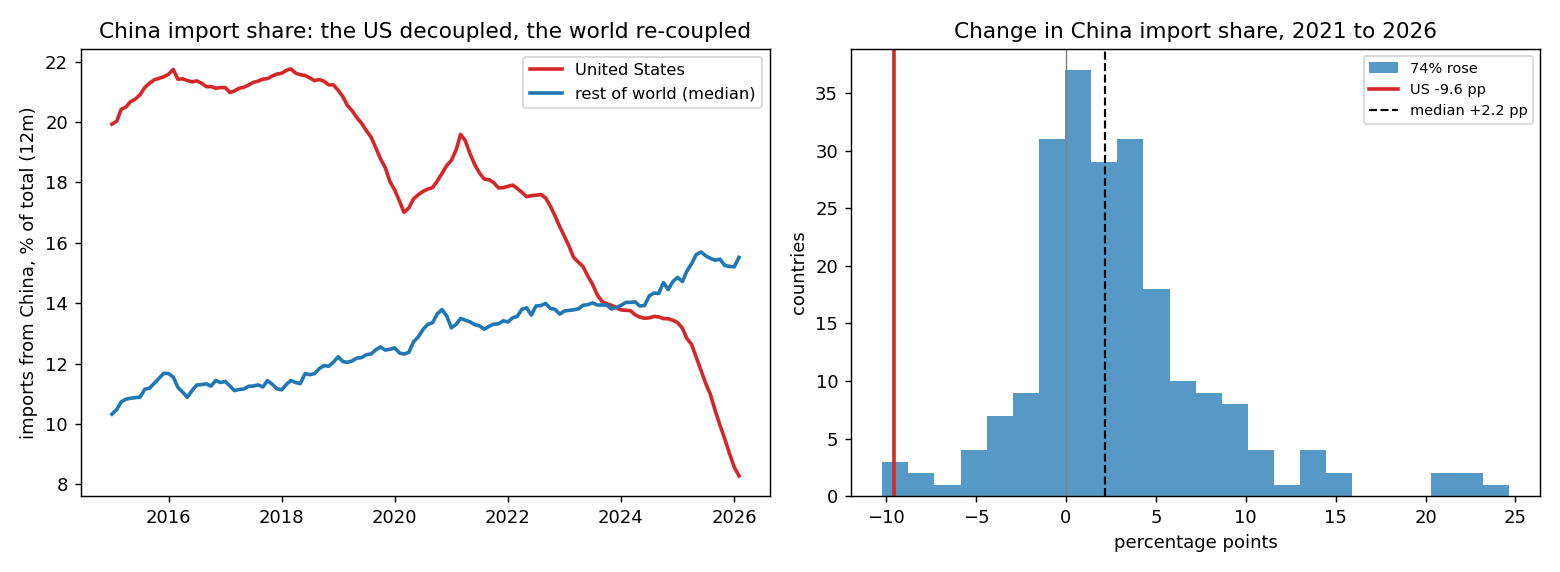
\includegraphics[width=\textwidth]{../output/figure1_china_shift.png} \caption{The world re-coupled to China; the United States decoupled. Left: the share of imports sourced from China, trailing twelve months, for the United States and the median of all other economies. The two series cross around 2023. Right: the change in each country's China import share between 2021 and 2026. The red line marks the United States, whose decline stands apart from the positive median across other economies.} \label{fig:facts} \end{figure} The bilateral data show a broad increase in dependence on China as a source of imports, accompanied by little change in China's role as a destination for exports. China's expanding productive capacity has supplied foreign economies with lower-cost goods and contributed to lower import prices. Its domestic market has absorbed a much smaller share of the exports on which those economies rely for income during downturns. For the countries examined in this paper, China's growing role in trade has therefore provided limited support through the external-demand channel studied here. Figure~\ref{fig:facts} summarizes the divergence. The Chinese share of US imports declined from about 20 percent to about 8 percent over the decade and fell below the median for the rest of the world around 2023. Over the same period, roughly three-quarters of other economies increased the share of their imports sourced from China. The literature on geoeconomic fragmentation identifies several channels through which changes in international integration can affect output, including trade, capital flows, migration, technology diffusion, and the provision of global public goods. Scenario-based estimates generally produce larger output losses under more extensive decoupling, with emerging and low-income economies bearing a disproportionate share of the burden \citep{aiyar2023, fv2024}. Those exercises describe paths in which cross-border integration recedes. The observed data over the period considered in this paper show continued growth in total trade alongside a substantial reallocation toward China. The income-group comparison leads to the same conclusion. After indexing each economy's goods trade to its average level in 2017--2019, median trade reached 131 among advanced economies, 134 among emerging and developing economies, and 149 among low-income economies during 2023--2025 (Table~\ref{tab:income}). Every income group had moved above its pre-pandemic level after recovering from the disruption of 2020--2022. Low-income economies recorded the largest increase relative to their own pre-pandemic baseline. Over this sample, changes in international integration were expressed mainly through the redirection of trade across partners. \begin{table}[H]
\centering\small
\caption{Goods trade with the world across three periods, median cumulative index by income group (stable pre-pandemic base 2017--2019 = 100): the shock transition (2020--2022) and the fragmentation period (2023--2025). Trade in every income group is well above its pre-pandemic level, and by more for emerging, developing, and low-income economies than for the advanced economies.}
\label{tab:income}
\begin{tabularx}{\textwidth}{@{}lYYYY@{}}
\toprule
Income group & Economies & 2017--19 & 2020--22 & 2023--25 \\ \midrule
Advanced & 35 & 100 & 112 & 131 \\
Emerging \& developing & 166 & 100 & 114 & 134 \\
Low income & 26 & 100 & 122 & 149 \\
\bottomrule
\end{tabularx}
\\[2pt]\footnotesize{\emph{Source:} IMF International Trade in Goods Statistics (IMTS), monthly. Trade is total goods trade with the world (imports CIF plus exports FOB). For each economy, average monthly trade in each period is indexed to its 2017--2019 average (=100); cells are the median across economies in each group. The 2020--2022 column spans the pandemic, the rebound, and the 2022 commodity-price spike. Groups are a rough classification into advanced, emerging and developing, and low-income economies.}
\end{table}
 The direction of that redirection has implications for recovery. China gained importance primarily as a producer, while the United States continued to serve as a major source of final demand. An economy may consequently trade more while becoming increasingly connected to a partner whose growth generates limited demand for its exports. Aggregate measures of fragmentation capture the broad reorganization of trade relationships. The bilateral data reveal the partner structure underlying that reorganization. The empirical analysis below shows that variation in this structure is associated with the pace of recovery, while total trade exposure carries little explanatory power on its own. Figure~\ref{fig:redirect} presents the same reallocation in levels. Annual US goods imports rose to approximately \$3.3 trillion, even as imports from China fell to about half their 2022 peak. Imports from Vietnam and Mexico expanded sufficiently to offset much of this decline, and their combined sales to the United States now exceed Chinese sales by more than a factor of two. China's annual goods exports, meanwhile, increased to approximately \$3.9 trillion. Most of this growth was absorbed outside the United States, with the rest of the world purchasing more than eight times the US amount. Aggregate trade volumes continued to expand as the bilateral routes connecting producers and markets changed substantially. \begin{figure}[t] \centering 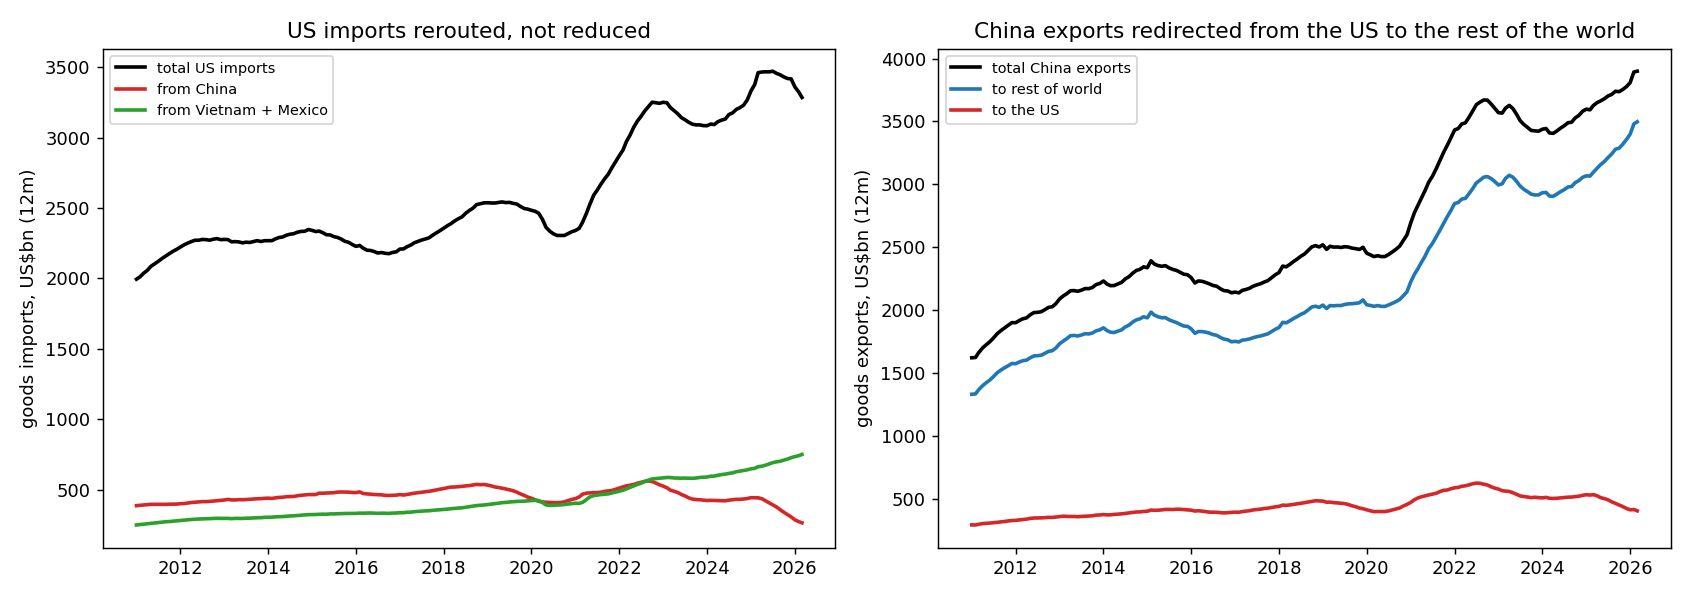
\includegraphics[width=\textwidth]{../output/figure_redirection.png} \caption{Trade growth and redirection, trailing twelve months. Left: total US goods imports increased as sourcing shifted away from China, whose sales fell to roughly half their 2022 peak, and toward Vietnam and Mexico, whose combined sales now exceed those of China by more than a factor of two. Right: China's total goods exports increased as destinations shifted toward the rest of the world, which now purchases more than eight times the amount sold to the United States.} \label{fig:redirect} \end{figure}

\section{A model of trade as risk sharing}\label{sec:theory}

\subsection{The risk-sharing mechanism}

Consider a small open economy $i$ whose output, in log deviation from trend, is a weighted sum of
what it sells at home and what it sells to a large core economy,
\begin{equation}
y_i = (1-s_i)\,\varepsilon_i + s_i\,\mu ,
\label{eq:portfolio}
\end{equation}
where $\varepsilon_i$ is an idiosyncratic domestic shock with variance $\sigma_\varepsilon^2$,
$\mu$ is the core's demand with variance $\sigma_\mu^2$, $\operatorname{cov}(\varepsilon_i,\mu)=0$,
and $s_i\in[0,1]$ is the share of $i$'s output sold to the core. Equation~\eqref{eq:portfolio}
is a portfolio: output places weight $1-s_i$ on a volatile own-income source and weight $s_i$ on
the core, so its variance is $\operatorname{Var}(y_i)=(1-s_i)^2\sigma_\varepsilon^2 +
s_i^2\sigma_\mu^2$. This is the standard portfolio view of international risk sharing, in which
selling to a steady partner diversifies idiosyncratic income risk \citep{obstfeld1994,
kalemliozcan2003}; the accompanying link between openness and output volatility, and its dependence
on structure, is documented by \citet{rodrik1998} and \citet{digiovanni2009}. The new element
here is the composition tilt $\theta$ introduced below.

Output variance $\operatorname{Var}(y_i)=(1-s_i)^2\sigma_\varepsilon^2+s_i^2\sigma_\mu^2$ is a
convex quadratic in the export share, minimized at
$s^\star=\sigma_\varepsilon^2/(\sigma_\varepsilon^2+\sigma_\mu^2)$, since
$\partial \operatorname{Var}(y_i)/\partial s_i =
2\,[\,s_i(\sigma_\varepsilon^2+\sigma_\mu^2)-\sigma_\varepsilon^2\,]$ is negative below $s^\star$
and positive above it. With zero covariance a marginal increase in exposure from zero lowers
variance for any finite $\sigma_\mu^2$, since the derivative at $s_i=0$ is $-2\sigma_\varepsilon^2<0$
whatever the relative volatilities. A steadier core, $\sigma_\mu<\sigma_\varepsilon$, simply raises
the variance-minimizing share above one half and enlarges the diversification gain. This is the
standard two-asset diversification result. The intuition is that selling to a
large, idiosyncratically uncorrelated consumer
provides insurance, because the consumer continues to purchase when the domestic shock materialises,
thereby diversifying $i$'s income. The condition that matters empirically is that the core's shocks
be \emph{uncorrelated} with $i$'s. Once the covariance enters, the derivative at $s_i=0$ becomes
$2(\operatorname{cov}(\varepsilon_i,\mu)-\sigma_\varepsilon^2)$, so exposure still lowers variance
as long as the covariance stays below $\sigma_\varepsilon^2$, and the diversification erodes and can
disappear only when the core's cycle coincides strongly with $i$'s. A consumer whose cycle moves
with $i$'s provides little insurance even when it is steady on its own. Steadiness is also in large part a policy
outcome: a partner that stabilizes its own economy, responding to downturns quickly enough that
its import demand recovers fast, delivers a low $\sigma_\mu$ to everyone who sells to it.

The core's absorption can be split into two components: import-intensive uses
(consumption and tradables), which draw in the periphery's goods, and
import-light ones (domestic services, structures, and non-traded capital), which do not. Let
$\theta$ be the share of absorption in the import-light component, so the demand the core directs
abroad declines with $\theta$ and $i$'s effective export share becomes $s_i(\theta)=
\omega_i(1-\theta)$, with $\omega_i$ the structural exposure. The tilt $\theta$ is a matter of
composition rather than technology, reflecting any shift of core spending toward goods and services
produced and consumed domestically. A shift of core spending toward domestically produced AI
services, a reshoring drive, and a defense build-out are all instances, and each would
raise $\theta$ in the same way.

\begin{corollary}\label{prop:tilt}
As the core spends a larger share of its absorption on import-light uses, so that $\theta$ rises
and the export share $s_i(\theta)$ falls below $s^\star$, the periphery's output variance rises,
\[
\partial\operatorname{Var}(y_i)/\partial\theta = -\omega_i\,\partial\operatorname{Var}(y_i)/\partial s_i>0.
\]
The core's own output can still rise as $\theta$ rises, since the import-light sector's output
counts in its GDP, even as the stabilization the core exports to the periphery falls.
\end{corollary}

Setting $\sigma_\varepsilon=5$ and $\sigma_\mu=2$, illustrative values chosen to display the
mechanism rather than estimated from the data, exposure to the core cuts output variance
by up to $86$ percent at $s^\star$, and the average periphery variance rises about $16$ percent
as $\theta$ moves from $0.2$ to $0.5$; the high-exposure economies, which are the most stabilized at
low $\theta$, lose the most (Figure~\ref{fig:layer1}). The magnitudes here are illustrative and the
qualitative comparisons do not depend on the particular values. A shift in the composition of core growth
toward import-light activity thus withdraws insurance from the periphery without any decline in core
output.

\begin{figure}[t]
\centering
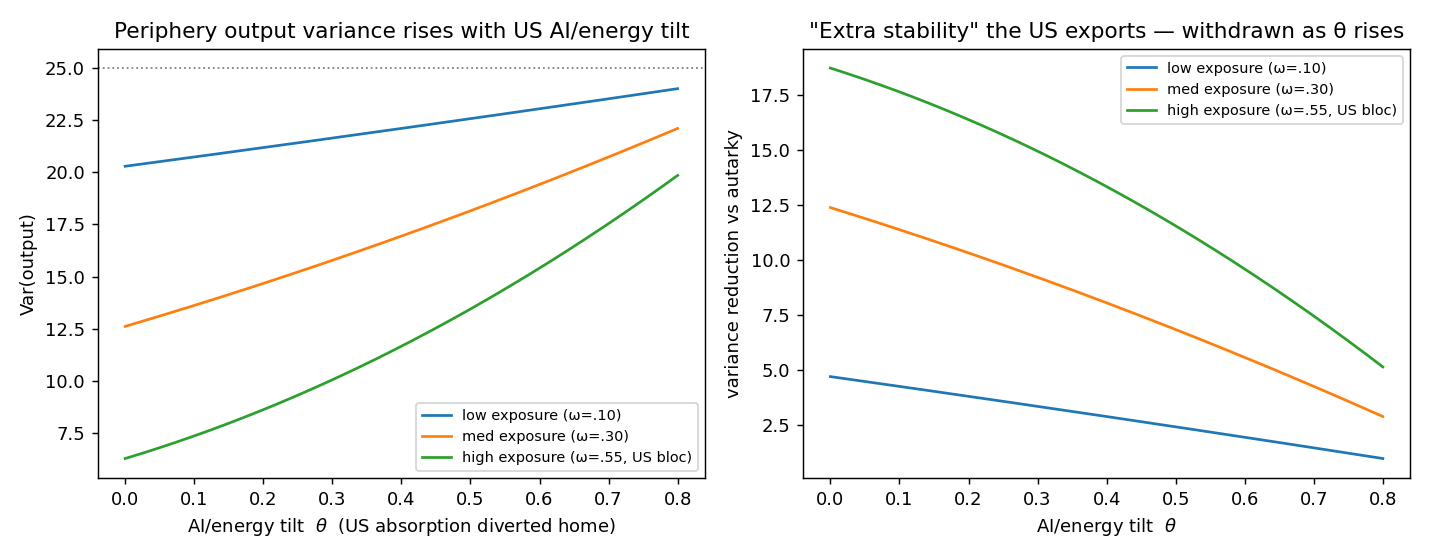
\includegraphics[width=\textwidth]{../output/model_layer1.png}
\caption{Trade as risk sharing. Left: periphery output variance rises with the import-light tilt
$\theta$, fastest for high-exposure economies. Right: the variance reduction that exposure to
stable core demand provides, withdrawn as $\theta$ rises.}
\label{fig:layer1}
\end{figure}

\paragraph{The riskiness of trade.} The model provides criteria for comparing trading partners. Demand from a partner
is good insurance when it is steady (low $\sigma_\mu$), uncorrelated with the client's own cycle,
and growing; and the relevant object is the partner's appetite for \emph{imports}, not its GDP,
since only imports pull a client's exports. Table~\ref{tab:partnerquality} scores the major hubs on
this dimension. Measured by import demand, the United States is the highest-quality anchor, its
demand growing at about 4 percent a year with the lowest volatility, for a quality ratio of $0.62$;
the European Union is steady but slow-growing ($0.30$); and China, though its import demand grows
fastest, is also the most volatile, so its quality ($0.43$) falls below that of the United States.
Ranking the hubs by GDP growth instead reverses the order and places China first, which is the
error the model warns against: China's growth generated limited import demand from the economies in
this sample, and in the model a partner's growth insures a trading partner only to the extent that it
is spent on that partner's exports. The empirical counterpart, which hub actually pulls a
client out of its own downturn, is examined empirically in Section~\ref{sec:results}.

\begin{table}[H]
\centering\small
\caption{Insurance quality of the major hubs' demand. Import demand, what pulls a client's exports, is steadiest and growing for the United States; China's grows but is twice as volatile. Ranking hubs by GDP growth instead (last column) misleads, placing China first, because China grew as a producer rather than a consumer.}
\label{tab:partnerquality}
\begin{tabularx}{\textwidth}{@{}lYYYY@{}}
\toprule
Hub & Import-demand & Volatility & Quality & GDP-growth \\
 & growth, \% & of demand, \% & (mean/vol.) & ratio \\ \midrule
United States & 4.2 & 6.7 & 0.62 & 2.57 \\
European Union & 3.1 & 10.2 & 0.30 & 1.25 \\
China & 5.6 & 13.0 & 0.43 & 3.77 \\
Japan & 1.2 & 12.2 & 0.10 & 1.01 \\
\bottomrule
\end{tabularx}
\\[2pt]\footnotesize{\emph{Source:} IMF IMTS (import demand, total goods imports from the world) and WEO (real GDP growth), 2010--2024 excluding the 2020 pandemic outlier. Import demand for the European Union aggregates its ten largest members. Quality is mean annual import growth divided by its standard deviation (computed from unrounded series); the GDP-growth ratio is mean annual real GDP growth divided by its standard deviation over the same window.}
\end{table}


\subsection{A dynamic illustration}
The portfolio result is static. To show how the composition of core growth affects recovery dynamically, we use a compact two-region gap model. The model is calibrated rather than estimated and is intended to illustrate one mechanism: two expansions that raise core output by the same amount can generate different paths abroad when their import content differs.

Core activity consists of import-intensive absorption, $\hat c_t$, and import-light domestic activity, $\hat q_t$. A small reduced-form stabilization rule, $\hat r_t=\phi_y\hat y_t^C$, moderates core activity but does not generate the cross-border ranking. Core output and imports are
\begin{align}
\hat y_t^C &= \omega_c\hat c_t+\omega_q\hat q_t, \\
\hat m_t &= \eta_c\hat c_t+\eta_q\hat q_t, \qquad \eta_c>\eta_q\geq0.
\end{align}
Thus both components can raise core output, but import-intensive absorption creates more foreign demand per unit of activity. Import-light activity may still raise imports, leave them broadly unchanged, or reduce them if it sufficiently displaces import-intensive absorption.

A peripheral economy receives the portion of core import demand associated with its predetermined bilateral exposure,
\begin{align}
\hat x_{i,t} &= \gamma_i\hat m_t,\\
\hat y_{i,t}^P &= \rho_P\hat y_{i,t-1}^P+\alpha\hat x_{i,t}+\varepsilon_{i,t}^P.
\end{align}
A negative domestic shock $\varepsilon_{i,t}^P$ generates a downturn, while external demand affects the subsequent path through exports. Recovery is defined as the first period in which peripheral activity returns to trend. The simulations compare import-intensive and import-light shocks normalized to produce the same impact increase in core output. An import-intensive expansion generates stronger imports and faster peripheral recovery, with a larger difference for economies whose bilateral exposure $\gamma_i$ is high. An import-light expansion provides less support and can delay recovery if it compresses core imports. Figure~\ref{fig:layer2} shows the calibrated responses, and Appendix~\ref{app:model} states the model, the proposition, and the calibration in full.

\begin{figure}[!htb]
\centering
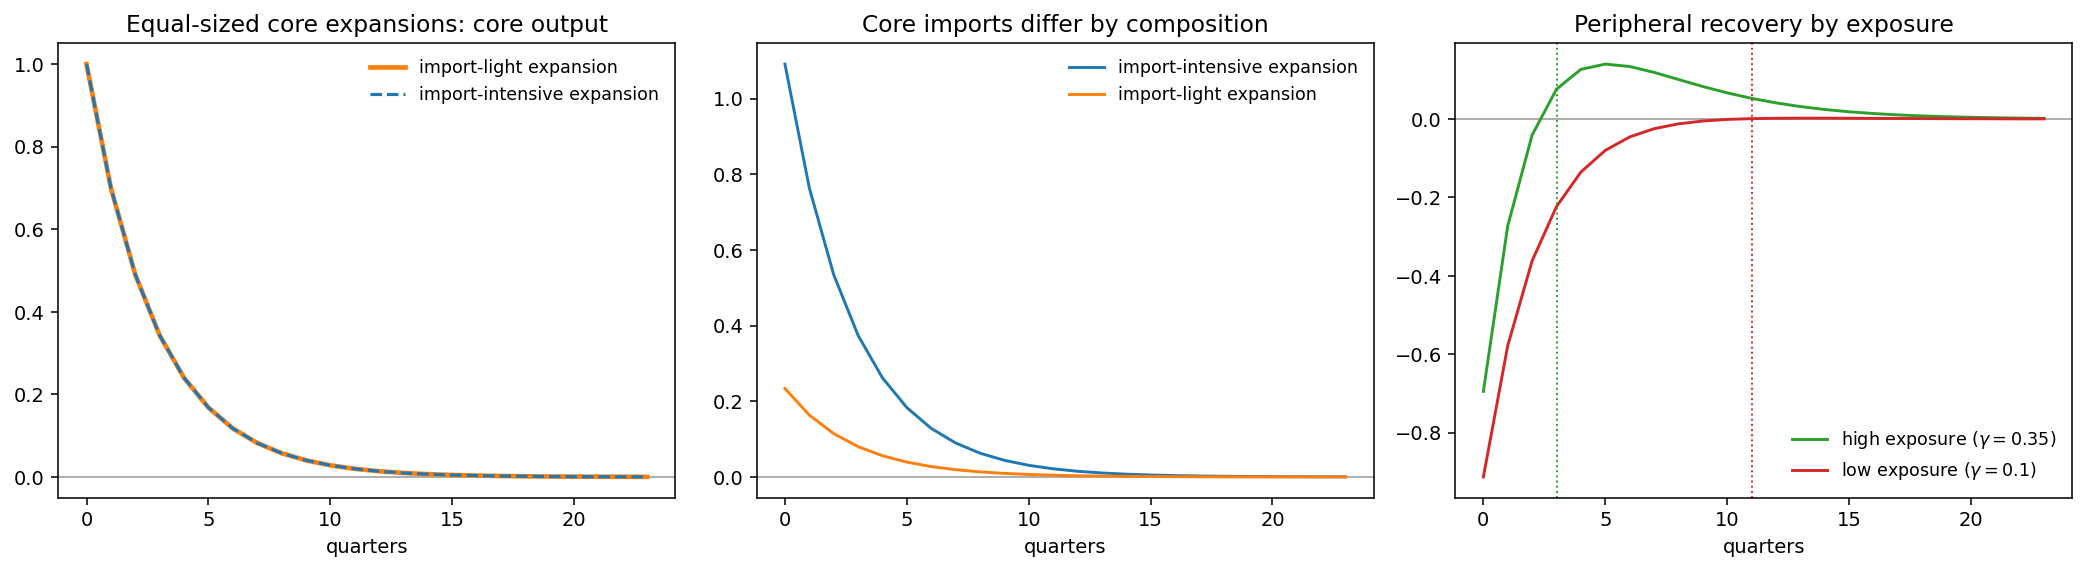
\includegraphics[width=\textwidth]{../output/model_layer2_irf.png}
\caption{Dynamic trade transmission under equal-sized core expansions. Left: core output under import-intensive and import-light shocks normalized to have the same impact effect. Centre: core imports, which differ because import-intensive absorption has greater import content. Right: peripheral recovery under low and high bilateral exposure to the core. The figure is a calibrated illustration rather than a quantitative estimate.}
\label{fig:layer2}
\end{figure}
\section{Data and empirical strategy}\label{sec:empirics}

\paragraph{Sample.} The paper studies economies with a demonstrated exposure to external
distress. As a sample frame we take the 97 countries with an IMF arrangement approved between 2005
and 2025, from the Monitoring of Fund Arrangements (MONA) database; requesting external financing
at some point over two decades marks an economy as exposed to the downturns the paper studies. The
same database records when an arrangement is active, which we track throughout so that the demand
effects are measured conditional on an active-arrangement indicator. For the recovery outcome we use high-frequency
activity indicators, since annual GDP is too coarse to date a recovery and quarterly GDP is missing for
most emerging markets. We assemble monthly central-bank activity indicators and industrial
production for 57 of these countries, seasonally adjusting the non-adjusted series with the
X-13ARIMA-SEATS procedure. The sample is best read as the population of externally exposed emerging
and developing economies with usable monthly activity data rather than as a convenience frame:
compared with other MONA economies and with emerging and developing economies that had no
arrangement in the window, the included economies are similar in average growth and trade openness,
modestly larger, and no more growth-volatile, while over-representing commodity exporters, a
difference the analysis controls for directly (Table~\ref{tab:samplecomp} in the appendix).

\paragraph{Episodes.} We date downturns endogenously from the Hodrick--Prescott (HP) output gap of
seasonally adjusted activity. Each spell during which the gap is negative and reaches a depth of
at least two percent is one episode. This yields 263 episodes across 34 countries over
2004--2024, far more than crisis-dating chronologies provide for these countries. Depth is the
absolute value of the most negative gap reached during the spell, so it is reported as a positive
magnitude. For each
episode we record the depth of the gap and three durations, the contraction (peak to trough),
the climb (trough to the gap's return to zero), and the full negative cycle (peak to the gap's
return to zero). Recovery is dated at the month the output gap returns to zero, so it marks a
return of activity to trend rather than to the exact pre-downturn level.

\paragraph{Demand measure.} The channel of interest is demand from partners that are growing. We
build a shift-share measure: for each episode, the trade-weighted average of partner real GDP
growth over a fixed window from the peak (the peak year and the two years following), with weights
the country's pre-downturn export shares. We
decompose it into the contribution of the United States, other advanced economies, emerging
markets excluding China, and China. The baseline measure uses the IMF's goods-trade database
(IMTS); because external demand also arrives through services and remittances, we complement it
with World Bank data on services exports, international tourism, and worker remittances in the
robustness of Section~\ref{sec:results}.

\paragraph{Specification.} We relate the depth and the durations to the demand measure, to
generic trade openness (trade over GDP), and to financial openness from the External Wealth of
Nations, with standard errors clustered by country. Every regression also tracks an indicator for
an active IMF-supported arrangement during the episode, from MONA, so the partner-demand associations
are estimated conditional on whether an arrangement is in place. The binary indicator does not
capture the size or intensity of a program, so it conditions on the presence of official support
rather than fully controlling for it.

\paragraph{Identification.}
The empirical analysis has two layers. The baseline episode-level specification is descriptive. It combines export shares fixed before the downturn with partner GDP growth measured from the peak year through the following two years. Predetermined shares prevent the recovery itself from changing the exposure weights, but they do not make subsequent partner growth an exogenous shock. In particular, the partner-growth window overlaps the recovery outcome, and common global or regional developments may raise both partner growth and domestic activity. The baseline coefficient is therefore interpreted as a conditional association rather than a causal effect.

The baseline analysis nevertheless contains several checks on the main confounding channels. The demand measure is decomposed by partner type; world growth excluding the United States, own-region growth, and peak-year fixed effects absorb common global and regional conditions; and the result is re-estimated using crisis-year partner growth, contraction duration, and monthly local projections. These exercises test whether the baseline association is a relabeling of the global cycle or an artifact of one recovery definition, but they do not by themselves supply quasi-experimental variation. Because the shifts are common across many episodes, the US shifter takes only about twenty distinct peak-year values and the effective number of independent country clusters is about twenty-two of the thirty-four, which is why inference is clustered by country and the result is confirmed under peak-year fixed effects.

A separate leave-one-out import-demand design provides a sharper validation. For episode $i$ with peak year $e$, define
\begin{equation}
Z_i=\sum_j s_{ij,e-1}g_{j,e}^{-i},
\label{eq:loo_shift}
\end{equation}
where $s_{ij,e-1}$ is the pre-downturn export share to destination $j$ and $g_{j,e}^{-i}$ is growth in destination $j$'s imports from all origins except economy $i$. Excluding economy $i$ from the destination's imports removes the direct mechanical feedback from its own exports into its measured foreign-demand shift. The shifts are also residualized with respect to destination and year effects, and inference is computed at the level of the underlying destination shocks, following the exposure-robust logic of \citet{adao2019} and the shock-level interpretation of \citet{borusyak2022}. Identification in this design requires the residualized destination import shifts to be orthogonal to unobserved determinants of economy $i$'s recovery, conditional on the included controls. The shares themselves need not be randomly assigned under this interpretation.

The leave-one-out design materially strengthens the case for an external-demand channel, but it does not eliminate every threat to causal interpretation. The available annual trade data do not contain destination-product cells, the import-growth window still overlaps part of the recovery, and destination shocks may affect the exposed economy through remittances, tourism, commodity prices, financial conditions, or confidence as well as through goods exports. Accordingly, the paper treats the leave-one-out estimates as quasi-experimental validation of the direction and partner structure of the baseline result, not as a fully isolated structural elasticity of recovery with respect to exports. Appendix~\ref{app:robust} reports the estimates, exposure-robust inference, balance tests, a pre-recovery placebo, and leave-one-destination diagnostics.
\section{Results}\label{sec:results}

The baseline estimates show that trading-partner demand is associated with recovery duration,
and for many of these economies that partner is the United States. Table~\ref{tab:main} reports the
decomposition of the demand measure by partner type across the depth of the downturn and its three
durations. Demand from advanced economies is associated with a shorter climb and a shorter full negative cycle, and
the association is concentrated in the United States, with the other advanced economies insignificant once
the US is separated out.\footnote{A Wald test of the equality of the US and other-advanced
coefficients on the full cycle gives a difference of $3.1$ months ($t=-1.9$, $p=0.07$), so the two
differ at the ten percent level rather than the US coefficient being merely more precisely
estimated.} The magnitude is economically large, and a one-percentage-point rise in
the US demand contribution is associated with a negative cycle roughly six months
shorter.\footnote{In the estimation sample the interquartile range of the US-demand contribution is
$0.8$ percentage points, so an interquartile increase is associated with a full cycle about
$4.7$ months shorter; the standardized effect is $0.25$ of a standard deviation.} The
contribution is the US export share times US growth rather than US growth itself, so a one-point
move in it is large relative to the range in the data; for a country with a ten percent US export
share it corresponds to about ten points of additional US growth, and the coefficient should be
read as the effect of a change in the export-share-weighted contribution rather than in US GDP
growth. Emerging-market demand contributes more modestly. The China term is positive and
significant for the depth and for the durations, so greater exposure to China is associated with
deeper and longer downturns rather than faster recoveries. The depth association is confined to
commodity exporters, shown below, and reflects the commodity cycle rather than any demand these
economies draw from China; the median export share to China in the sample is below half a percent,
too small for Chinese final demand to reach them. This is the export-side counterpart of the
import-side shift documented in Section~\ref{sec:facts}. Partner growth is averaged over a fixed
window anchored at the peak, which overlaps the recovery it explains, so part of the association
could be timing-driven; measuring partner demand only in the crisis year substantially shortens the
overlap relative to the three-year window, though it is not strictly predetermined when a downturn
begins before the end of the calendar year, and this measure leaves the US effect intact, while the
contraction result and the local projections, where the timing is cleaner, confirm it.\footnote{The onset measure, which
uses only the crisis-year value of partner growth, gives a US full-cycle coefficient of $-3.8$
($t=-4.1$); see Table~\ref{tab:prewindow} in the appendix.}

\begin{table}[t]
\centering
\small
\caption{External demand and the output cycle, by partner type. Output-gap episodes, country-clustered standard errors ($t$ in parentheses).}
\label{tab:main}
\begin{tabular}{lcccc}
\toprule
 & Depth & Contraction & Climb & Full cycle \\
\midrule
US demand & $-0.79$ {\scriptsize$(-0.6)$} & $-2.23^{***}$ {\scriptsize$(-3.1)$} & $-3.60^{***}$ {\scriptsize$(-3.2)$} & $-5.59^{***}$ {\scriptsize$(-3.6)$} \\
Other advanced demand & $3.66$ {\scriptsize$(1.6)$} & $-0.07$ {\scriptsize$(-0.1)$} & $-2.72^{**}$ {\scriptsize$(-2.3)$} & $-2.53^{*}$ {\scriptsize$(-1.9)$} \\
Emerging demand (excl.\ China) & $-0.54$ {\scriptsize$(-0.7)$} & $-0.23$ {\scriptsize$(-0.7)$} & $-1.13$ {\scriptsize$(-1.5)$} & $-1.28$ {\scriptsize$(-1.5)$} \\
China demand & $2.25^{***}$ {\scriptsize$(3.6)$} & $-0.21$ {\scriptsize$(-0.6)$} & $2.57^{***}$ {\scriptsize$(3.6)$} & $1.86^{**}$ {\scriptsize$(2.1)$} \\
Trade openness & $0.31$ {\scriptsize$(0.2)$} & $1.10$ {\scriptsize$(1.2)$} & $-0.22$ {\scriptsize$(-0.1)$} & $0.60$ {\scriptsize$(0.3)$} \\
Partner volatility & $1.63^{***}$ {\scriptsize$(3.2)$} &  &  &  \\
Depth of downturn &  & $0.10^{***}$ {\scriptsize$(3.3)$} & $0.26^{***}$ {\scriptsize$(3.5)$} & $0.35^{***}$ {\scriptsize$(4.7)$} \\
\midrule
Episodes & 263 & 263 & 263 & 263 \\
Countries & 34 & 34 & 34 & 34 \\
\bottomrule\end{tabular}
\\[2pt]\footnotesize{Depth in percent; durations in months. Contraction is peak (start of the negative-gap spell) to trough (minimum gap), climb is trough to the output gap's return to zero, full cycle is peak to the output gap's return to zero. All columns also track official support with an indicator for an active IMF-supported arrangement (MONA), so the demand effects are estimated conditional on whether an arrangement is in place. $^{*},^{**},^{***}$: significant at 10, 5, 1 percent.}
\end{table}

\begin{table}[t]
\centering
\small
\caption{The China-depth association is commodity-exporter composition.}
\label{tab:china}
\begin{tabular}{lc}
\toprule
 & Depth of downturn \\
\midrule
China demand $\times$ commodity exporter & $1.73^{***}$ {\scriptsize$(4.4)$} \\
China demand $\times$ non-commodity & $-4.50$ {\scriptsize$(-1.3)$} \\
Commodity exporter & $-1.74$ {\scriptsize$(-1.0)$} \\
Emerging demand (excl.\ China) & $-1.23^{**}$ {\scriptsize$(-2.4)$} \\
Other advanced demand & $2.03$ {\scriptsize$(0.9)$} \\
US demand & $-3.16^{***}$ {\scriptsize$(-2.8)$} \\
Trade openness & $-0.41$ {\scriptsize$(-0.2)$} \\
\midrule
Episodes & 263 \\
Countries & 34 \\
\bottomrule\end{tabular}
\\[2pt]\footnotesize{China demand interacted with a commodity-exporter indicator. The effect is present only among commodity exporters. The regression also tracks an indicator for an active IMF-supported arrangement.}
\end{table}


Generic trade openness has no statistically detectable association with the depth or the duration
of a downturn. Its coefficients are positive in the depth and contraction regressions and small in
the durations, and none of them is significant (Table~\ref{tab:main}). Openness measures how much a
country trades, whereas the demand measure captures whether its partners are growing, and only the
second is associated with the speed of recovery.

The volatility of a country's partners, measured as the exposure-weighted standard deviation of
their growth, enters the depth regression positively and significantly, so an economy tied to
volatile partners falls further, because a volatile partner cycle is transmitted to it. A distressed
economy benefits from partners that are large, growing, and steady, while one that is remote from
growth and exposed to volatile partners faces the most difficult adjustment.

The steadiness of a partner is largely a policy outcome, and this can be measured directly. We
build a fully predetermined measure of partner stabilization quality, the export-share-weighted
average of each partner's rebound strength, its growth in the year after its own negative-growth
years, computed on data through the episode's peak year only. On its own, this predetermined
characteristic predicts a shorter cycle and a shallower fall, both at the margin of significance;
adding the realized demand pulls absorbs it while the US term stays significant
(Table~\ref{tab:stabilization} in the appendix). That ordering follows from the mechanism, since
a partner's stabilization capacity matters because it delivers demand when the demand is needed,
so the trait predicts recovery until the demand it delivers is measured directly. Because the
measure is predetermined, it is also free of the timing concern attached to the demand window.

Exposure to China is associated with deeper downturns in the raw data (Table~\ref{tab:main}, depth
column), but splitting the China term by exporter type (Table~\ref{tab:china}) shows the
association is confined to commodity exporters. The interaction with a commodity-exporter indicator
is positive and strongly significant, while for non-commodity economies the term is insignificant
and wrong-signed. The pattern reflects the commodity cycle rather than a destabilizing effect of
China on diversified economies. This decomposition is estimated for the depth. Whether
commodity-exporter composition also explains the positive China coefficients for the climb and the
full cycle is not examined here.

\subsection{Recovery through regional hubs}

Leaving out any single country moves the US coefficient only modestly, so no one outlier drives
it, but dropping the six most US-exposed economies together collapses it to zero.\footnote{The
leave-one-country-out US full-cycle coefficient ranges from $-5.2$ to $-6.6$. The number of
episodes per country is uneven, with Costa Rica contributing 29 and several economies one; weighting
each country equally, by the inverse of its episode count, leaves the US full-cycle coefficient at
$-8.4$ ($t=-4.5$), so the many-episode economies attenuate rather than manufacture the result.} A shift-share
estimate works this way by construction \citep{goldsmith2020}, since it is identified off the units
that actually trade with the hub. Concentration is not the same as fragility, and a randomization
test separates the two. Permuting the US export-share vector across economies at random, while
holding US growth fixed to each episode's window, and re-estimating, the true coefficient is larger
in magnitude than every one of 2{,}000 placebo reassignments (randomization $p<0.001$). The
estimate therefore depends on the observed allocation of US export exposure across economies rather
than on the common variation in US growth alone (Figure~\ref{fig:placebo}).

\begin{figure}[t]
\centering
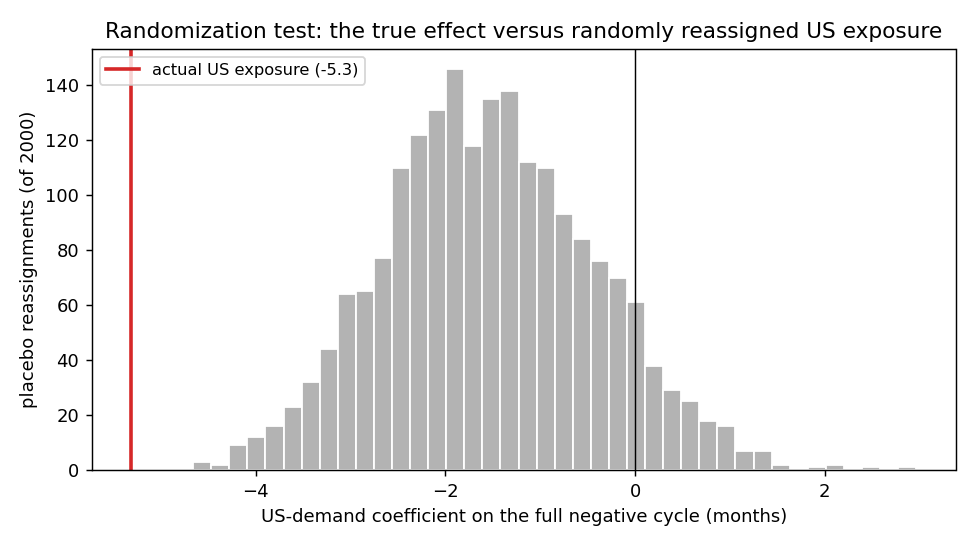
\includegraphics[width=0.8\textwidth]{../output/figure_placebo.png}
\caption{Randomization test on the exposure shares. The histogram is the US-demand coefficient on
the full negative cycle under 2{,}000 random permutations of the US export-share vector across
economies, holding US growth fixed to each episode's window; the red line is the estimate under the
actual exposure. The true coefficient is more negative than every placebo (randomization
$p<0.001$), so the association is driven by the real structure of US exposure rather than by which
economies happen to recover. The placebo distribution is centered near $-1.5$ rather than zero
because US growth co-moves with the global cycle, a timing component available to any random
assignment of exposure; the distance from that centre to the actual estimate is the part only
the true exposure structure produces. The test rebuilds the pull as the exposure share times US
growth in a parsimonious specification, so its coefficient differs slightly from the full
decomposition of Table~\ref{tab:main}.}
\label{fig:placebo}
\end{figure}

We therefore test the hub structure directly. Each country is assigned to the hub it exports
most to, the United States, the European Union, or China, and we estimate how strongly each
bloc's own hub pulls its recovery.

The countries sort into clear groups: nine export mostly to the United States (Mexico, Central America,
Colombia, Ecuador), twenty-four mostly to Europe (emerging Europe, and commodity exporters such
as Argentina, Chile and Peru), and exactly one, Mongolia, mostly to China.\footnote{Assignment
uses the pre-downturn export shares of each economy's episodes, so it reflects the trade
structure prevailing before each downturn rather than today's. Chile's episode peaks in 2008 and
Peru's in 2004--2013, before China displaced the European Union as their main destination, which
is why both sit in the Europe bloc; on current shares they would sort toward China.} The split by
bloc is sharp. The US-linked economies recover through US demand, at $-4.9$ ($t=-4.1$), and the
Europe-linked economies recover through European demand, at $-2.5$ ($t=-1.9$). The European effect
is weaker and only marginally significant, because the European hub grew more slowly over the
period, so the anchor has to be a \emph{growing} partner to pull. Pooling the two blocs into a
single own-hub term blurs the pattern, since it averages a fast-growing US hub with a slow-growing
European one, so the pooled own-hub pull is no larger than the pull from non-hub partners.\footnote{On
the full cycle the pooled own-hub coefficient is $-1.5$ ($t=-1.0$) against $-1.3$ ($t=-1.8$) for
non-hub demand.}

The bloc-specific estimates indicate that recovery is associated with demand from the hub to which an economy is most closely linked,
and the United States is simply the strongest such hub, closely linked and fast-growing. China, by
contrast, is not an export hub for this sample: no economy other than Mongolia sells mostly to it,
so an export-side China hub cannot be estimated here at all. The absence is informative for this
sample: over this period China grew as these economies' supplier rather than as a market for their
exports. It is the export-side counterpart of the import-side shift in Section~\ref{sec:facts}, and
it is why, for the economies studied here, the eastward re-coupling has not supplied a new recovery
anchor.

The hub structure also identifies which economies face the most difficult adjustment. A hub is
defined not by being advanced or stable in the abstract but by being large, close, and growing: the
model's stabilizing share $s_i$ is high only when a growing anchor is nearby, and gravity keeps that
share low for remote economies. Proximity to a stable but stagnant partner provides little support,
which is why the European hub pulls weakly. The most difficult case is therefore an economy with no
large, growing consumer within reach and volatile partners in its place, the isolated commodity
exporter tied to a fluctuating cycle. Distance from stable demand is, in effect, distance from
growth, and it leaves an economy without a route to recovery.

\paragraph{Inference and robustness.} With only 34 clusters the cluster-robust standard error could
over-reject, so we also compute a restricted wild cluster bootstrap \citep{cameron2008}, which
confirms the US coefficient at $p<0.001$. Country clustering allows for repeated episodes within a
country, but the same US growth realization enters every episode sharing a peak year, so we also
cluster on country and peak year jointly \citep{cameron2011}, which allows for dependence across the
economies that face a common shifter in a given year. The two-way standard error is only slightly
wider than the country-clustered one and leaves the US full-cycle coefficient significant at the one
percent level.\footnote{The two-way (country by peak-year) clustered standard error on the US
full-cycle coefficient is $1.7$, against $1.6$ under country clustering alone, giving $t=-3.4$
($p=0.003$).} The estimate is stable across the natural perturbations of
the design. Because the depth of the downturn is itself an outcome, and part of the US-demand
effect may run through a shallower downturn, controlling for depth could absorb part of the effect
and bias the estimate toward zero. Dropping the depth control makes the US coefficient somewhat
larger rather than smaller, so the control if anything understates the demand association. The
overlap between the partner-growth window and the recovery is reduced by the contraction duration,
which overlaps less of that window than the full-cycle duration does and gives a similar US effect,
so it reduces but does not eliminate the timing concern. Replacing the two-sided filter with a
one-sided, real-time filter, restricting to the 25 episodes that coincide with a recognized
Laeven-Valencia crisis, and varying the depth threshold between 1.5 and 3 percent all leave the US
coefficient negative. The China coefficient is less stable, positive and significant in the baseline
and the lower-threshold specification, insignificant under the one-sided filter, and imprecisely
estimated in the crisis subsample.\footnote{US full-cycle
coefficients: dropping the depth control, $-6.6$ ($t=-4.1$); the contraction duration, $-2.1$
($t=-3.4$); the one-sided filter, $-7.1$ ($t=-3.4$). The depth-threshold and crisis-subsample
specifications are reported in Table~\ref{tab:robustness}.}

A further concern is the commodity price cycle. Commodity prices co-move with global
growth, and many sample economies export commodities, so partner demand could in principle proxy a
commodity boom. We therefore add each country's own commodity terms-of-trade impulse, the growth of
the IMF Commodity Net Export Price Index with fixed weights \citep{gruss2019}, measured over the
same window as the demand measure and interacted with the commodity-exporter indicator
(Table~\ref{tab:commodity} in the appendix). The impulse is nearly orthogonal to US demand in this
sample, and controlling for it leaves the US coefficient essentially unchanged on both the full
cycle and the contraction, while the commodity impulse itself has no significant effect on any
duration.\footnote{The correlation between the commodity impulse and US demand is $0.03$. With the
impulse included, the US coefficient is $-5.6$ ($t=-3.6$) on the full cycle and $-2.2$ ($t=-3.1$)
on the contraction.} The stability of the coefficient suggests that the US-demand association is not explained by the measured commodity terms-of-trade channel.

\paragraph{Censored recovery durations.} The full negative cycle is a time-to-event outcome, and
the eight episodes that never return to trend within the sixty-month window are top-coded rather
than observed, so the linear regression could in principle misstate the effect. We therefore
re-estimate recovery as a censored duration. Kaplan-Meier curves split at the median US-demand
pull show the high-exposure group returning to trend faster throughout the window, and a
discrete-time proportional-hazards model that treats the non-recovering spells as right-censored
gives a US-demand hazard ratio well above one, with the other partner pulls insignificant. The
censored-duration estimates reproduce the sign, the concentration in the US term, and the
significance of the linear duration regressions (Figure~\ref{fig:km} and
Table~\ref{tab:survival}).\footnote{The high-exposure group has a median recovery of four months
against eight for the low-exposure group, and a log-rank test rejects equality of the two curves at
$p<0.001$. In the discrete-time hazard model, fit with a complementary-log-log link and
country-clustered standard errors, the US-demand pull carries a hazard ratio of $2.25$ ($z=4.3$),
so a one-percentage-point increase in the US pull more than doubles the monthly probability of
returning to trend.}

\paragraph{Recovery measures independent of the HP crossing.} Episode selection, depth, and the
recovery date all derive from the same output gap, and a brief crossing of zero can date a recovery
that does not hold. We therefore re-estimate the decomposition on two outcomes that do not depend on
the crossing: a persistent-return duration, which dates recovery only once the gap stays
non-negative for three or six months, and cumulative activity loss, the area of the negative gap
over the episode, which has no crossing date at all (Table~\ref{tab:altrecovery}). The central
association survives. External demand from all partners is associated with a shorter persistent-return
cycle at the three-month horizon ($-1.5$, $t=-2.0$), demand from advanced economies more strongly so
($-3.0$, $t=-2.2$), and the US-demand pull dominates cumulative activity loss ($t=-3.7$), where a
stronger pull is associated with a smaller loss. The concentration in the US term is, however,
sensitive to how recovery is dated. Once a recovery must persist for three months, the
advanced-economy association spreads across the United States and the other advanced partners rather
than resting on the US alone, and the US point estimate loses significance on the persistent-return
duration while staying large on the magnitude margin. The six-month figure is therefore best read as
the association on the baseline crossing rather than as a definition-free constant, and the robust
statement is the narrower one: recovery is faster when the advanced markets an economy already sells
to keep growing. The six-month persistence column is imprecise, because requiring six clear months
late in the sample right-censors about a tenth of the episodes, and we do not lean on it.

\subsection{A portfolio reweighting calculation}

The hub structure invites a simple quantification of what a different portfolio of partners would
be worth, in months of downturn. We rebalance each economy's pre-crisis export-share vector and price the
change with the full-cycle coefficients of Table~\ref{tab:main}, at the partner growth each
episode actually faced. Moving five percentage points of the portfolio toward the economy's own
hub, funded proportionally from all non-hub partners, saves the median US-linked economy about
half a month of negative cycle per episode (median $-0.5$, interquartile range $-0.6$ to
$-0.3$), and the exercise is linear in the size of the shift, so a ten-point reorientation is
worth about a month per episode. For the Europe-linked economies the same rebalancing saves
nothing, with a median near zero, because over this period their hub grew more slowly than the
emerging partners that would fund the shift, so tilting further toward a slow-growing hub does
not shorten the downturn. When the shift is funded specifically out of the China share rather than
from all non-hub partners, both blocs save about half a month, since moving exposure away from a
destination that buys little and toward any growing hub helps regardless of bloc
(Table~\ref{tab:counterfactual}).

\begin{table}[H]
\centering\small
\caption{A partner-portfolio counterfactual: months of full negative cycle saved by moving five percentage points of the pre-crisis export-share portfolio, priced with the full-cycle coefficients of Table~\ref{tab:main} at each episode's realised partner growth. Negative values are months saved. An accounting exercise with local, partial-equilibrium coefficients, not a general-equilibrium prediction.}
\label{tab:counterfactual}
\begin{tabularx}{\textwidth}{@{}lYYY@{}}
\toprule
Rebalancing & Episodes & Median months & Interquartile range \\ \midrule
Toward own hub, all economies & 219 & $-0.0$ & $[-0.3,\ 0.1]$ \\
\quad US-hub economies & 69 & $-0.5$ & $[-0.6,\ -0.3]$ \\
\quad EU-hub economies & 146 & $0.0$ & $[-0.1,\ 0.1]$ \\
\midrule
From China to own hub (China share $>0.5$\%) & 167 & $-0.4$ & $[-0.7,\ -0.2]$ \\
\quad US-hub economies & 60 & $-0.5$ & $[-0.8,\ -0.3]$ \\
\quad EU-hub economies & 107 & $-0.4$ & $[-0.7,\ -0.2]$ \\
\bottomrule
\end{tabularx}
\\[2pt]\footnotesize{The move toward the hub is funded proportionally from all non-hub partners (upper panel) or from the China share alone, capped at that share (lower panel). The 219 observations in the upper panel correspond to the 219 unique country-by-peak-year export portfolios across the 263 episodes (69 US-hub, 146 EU-hub, and 4 China-hub in Mongolia); the lower panel restricts to the 167 portfolios with a pre-downturn China export share exceeding 0.5 percent (excluding China-hub episodes).}
\end{table}


The calculation shows that reweighting the
portfolio toward a hub raises recovery speed only when that hub is growing. It also locates where
the large differences come from.
A five-point shift buys half a month, so the several-month gaps in recovery speed across
economies reflect deep, structural differences in orientation, of the kind that distinguish an
economy selling half its exports to a growing hub from one remote from any, rather than marginal
reallocations. These are accounting magnitudes, computed from local coefficients at fixed prices;
they size the estimates and are neither a general-equilibrium prediction nor a recommendation to
redirect trade by policy.

\subsection{Services and remittances}

The demand measure is built from goods trade, for which bilateral partner-level data exist.
Services exports, tourism, and worker remittances operate through the same channel: a foreign
consumer whose demand continues in a downturn. In some economies, including Sri Lanka, these
flows dominate the recovery. However, bilateral partner data for services are unavailable, so a
fully bilateral services shift-share cannot be constructed. We therefore use country-level
intensities from the World Bank and report three checks (Table~\ref{tab:services}).

First, controlling for the intensity of remittances, services exports, and tourism leaves the
goods result essentially unchanged, and the intensities are individually insignificant
(Table~\ref{tab:services}, column 1). The goods measure is therefore not a proxy for services
reliance. Second, the US-demand association is similar for services-dependent economies, where the
interaction is insignificant. For the most remittance-dependent economies there is weak evidence,
at the margin of significance, of a smaller effect (column 2), which is expected when external
income arrives through remittances rather than goods exports. Third, a broader measure that adds
services and remittance intensity, weighted by advanced-partner growth, to the goods shift-share
also predicts a shorter cycle (column 3). The recovery channel is therefore external demand in
general, of which goods trade is the component that can be measured bilaterally.

\begin{table}[H]
\centering\small
\caption{External demand beyond goods: services and remittances. The dependent variable is the full negative cycle in months; country-clustered $t$-statistics in parentheses. Column 1 adds World Bank intensity controls to the goods partner-demand specification; column 2 interacts US demand with top-tercile services and remittance dependence; column 3 replaces the goods shift-share with a broad measure that augments it with the services- and remittance-intensity-weighted growth of advanced partners.}
\label{tab:services}
\begin{tabularx}{\textwidth}{@{}lYYY@{}}
\toprule
 & (1) controls & (2) heterogeneity & (3) broad demand \\ \midrule
US / goods partner demand & $-6.53^{***}$ {\scriptsize$(-5.2)$} & $-7.57^{***}$ {\scriptsize$(-3.6)$} &  \\
Broad external demand &  &  & $-0.87^{*}$ {\scriptsize$(-1.8)$} \\
US demand $\times$ high services &  & $-0.18$ {\scriptsize$(-0.1)$} &  \\
US demand $\times$ high remittances &  & $1.91$ {\scriptsize$(1.1)$} &  \\
Emerging partner demand & $-2.11^{***}$ {\scriptsize$(-2.6)$} & $-2.12^{**}$ {\scriptsize$(-2.6)$} &  \\
Trade openness & $2.10$ {\scriptsize$(0.7)$} & $0.31$ {\scriptsize$(0.1)$} & $4.20$ {\scriptsize$(1.1)$} \\
Remittances, \% GDP & $0.01$ {\scriptsize$(0.1)$} &  &  \\
Services exports, \% GDP & $-0.09$ {\scriptsize$(-1.1)$} &  &  \\
Tourism, \% of exports & $-0.06$ {\scriptsize$(-0.9)$} &  &  \\
\midrule
Episodes & 263 & 263 & 263 \\
Clusters & 34 & 34 & 34 \\
\bottomrule
\end{tabularx}
\\[2pt]\footnotesize{Intensities are pre-downturn values from the World Bank WDI (remittances received, services exports, international tourism receipts). Bilateral partner data for services are unavailable, so the broad measure proxies the source of services and remittance income by advanced-partner growth; the goods component is the bilateral shift-share of the baseline.}
\end{table}


\subsection{The response to a US-demand impulse}

To trace the same pattern month by month, we estimate state-dependent local projections (LP) of
activity on a Bartik US-demand impulse: the twelve-month growth of US industrial production
scaled by each country's export share to the United States.\footnote{The regressions include
country fixed effects, the level of the output gap, the recession-state indicator, and two lags
of monthly activity growth; standard errors are clustered by country, and the impulse is
standardized to unit variance.} The states are cyclical phases rather than month-by-month signs.
A month counts as in recession when its gap is below $-0.2$ percent within a continuous
below-trend spell of business-cycle length, one to seven years, and as normal when the gap is
above $+0.2$ percent. Months on trend, in transitory dips, or in implausibly long spells are
ambiguous and excluded, so noise in the series does not switch the state. The impulse raises
activity in both states (Figure~\ref{fig:lp}, Table~\ref{tab:lp}). In normal times the response
peaks at about 1.5 percent after eight to nine months. In a downturn it builds more slowly and
persistently, reaching 0.7 percent and still rising at eighteen
months.\footnote{The peak response is 1.5 percent (SE 0.24, $t=6.1$) in normal times; the
recession response at eighteen months is 0.7 percent (SE 0.24, $t=3.0$).} The positive
transmission of US activity is consistent with the episode-level result, observed month by month. Classifying
instead by the plain sign of the gap, which lets transitory dips count as recessions, preserves
both shapes with a weaker recession response.\footnote{At the terminal horizon the recession
response is $0.60$ under the sign rule against $0.73$ under the baseline classification.}

\begin{figure}[t]
\centering
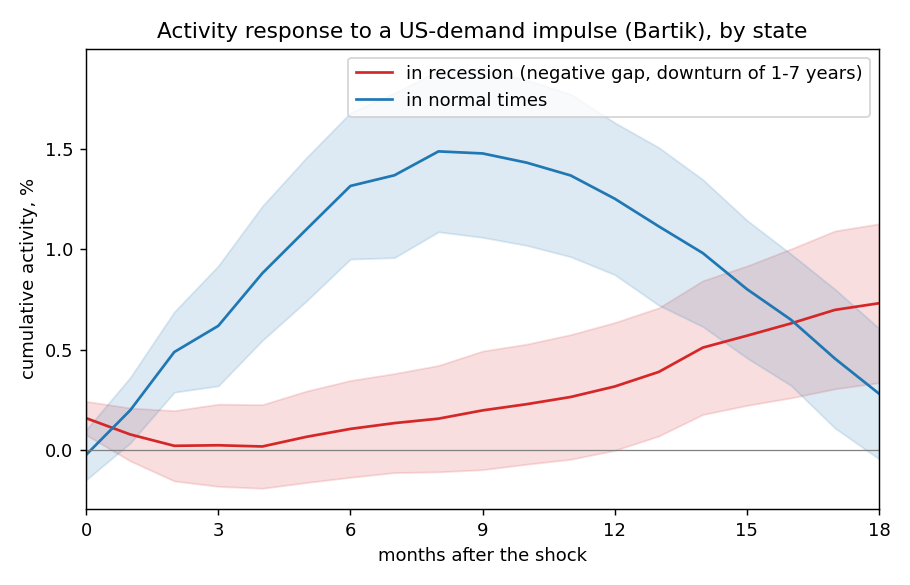
\includegraphics[width=0.75\textwidth]{../output/local_projections.png}
\caption{State-dependent local projections. Cumulative activity response to a one standard
deviation US-demand impulse, in recession (a negative output gap within a continuous downturn of
one to seven years) and in normal times (gap above trend); on-trend and transitory-dip months are
excluded. Bands are 90 percent, country-clustered.}
\label{fig:lp}
\end{figure}

\begin{table}[H]
\centering\small
\caption{State-dependent local projections: cumulative activity response to a one-standard-deviation US-demand (Bartik) impulse, by horizon and state. Country fixed effects; standard errors clustered by country in parentheses. $^{*}/^{**}/^{***}$: 10/5/1\%.}
\label{tab:lp}
\begin{tabularx}{\textwidth}{@{}lYYYYY@{}}
\toprule
Horizon (months) & 0 & 3 & 6 & 12 & 18 \\ \midrule
Normal times & -0.02 & 0.62$^{***}$ & 1.31$^{***}$ & 1.25$^{***}$ & 0.28 \\
 & (0.08) & (0.18) & (0.22) & (0.23) & (0.20) \\
In recession & 0.16$^{***}$ & 0.03 & 0.11 & 0.32$^{*}$ & 0.73$^{***}$ \\
 & (0.05) & (0.12) & (0.15) & (0.19) & (0.24) \\
\bottomrule
\end{tabularx}
\end{table}


\subsection{Hub growth in local and global downturns}

The value of an anchor depends not on its average growth but on its growth \emph{during the
country's own downturn}. A hub that continues to purchase while a country is in downturn supports
its recovery; one that contracts alongside it does not. Figure~\ref{fig:chances} measures this: for
each country, the growth of its hub over the recovery window of its own local downturns, with the
global-crisis years 2008, 2009 and 2020 removed. In a local downturn the hub is almost always
growing, with a median of 1.9 percent, so the anchor is there when it is needed; and the US-linked
economies have the strongest anchor of all, their hub growing around 2.5 percent while the
Europe-linked economies get only 1 to 1.5. Linkage to the United States is an advantage in a
local crisis; pooling all episodes understates that advantage, because the global-crisis years,
in which Mexico and the United States contracted together, pull the average down.

\begin{figure}[t]
\centering
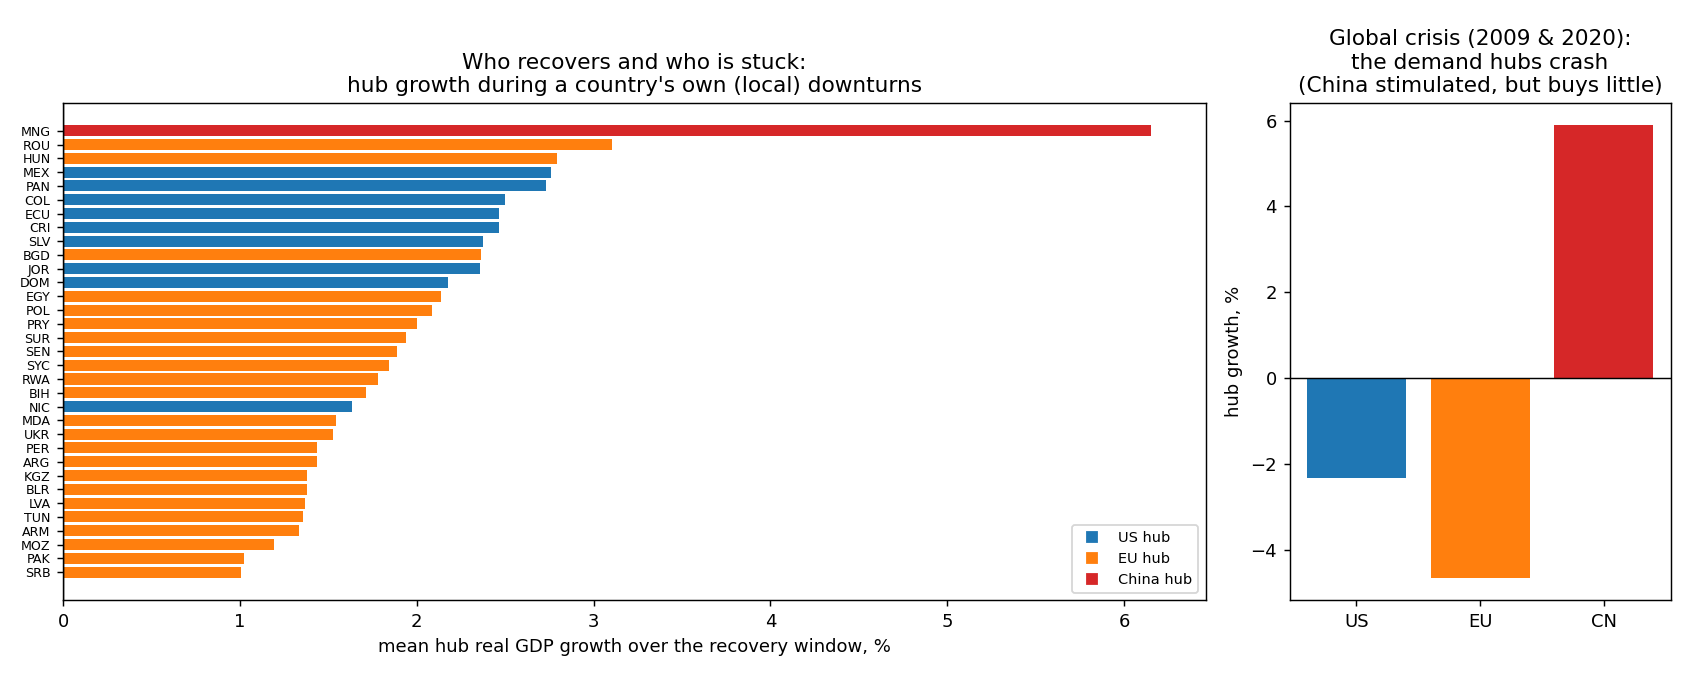
\includegraphics[width=\textwidth]{../output/recovery_chances.png}
\caption{Left: mean hub real GDP growth over the recovery window of each country's own local
downturns (global-crisis years excluded), coloured by hub. In a local crisis the anchor is
present, and strongest for the US-linked bloc. Right: in a global crisis the demand hubs both
contract, so the anchor fails; China grew through 2009 and 2020, but it buys too little from these
economies to substitute.}
\label{fig:chances}
\end{figure}

However, the mechanism has a limit in a global crisis. The channel insures against
\emph{idiosyncratic} downturns and does not operate when the downturn is global. In
2009 and 2020 both demand hubs contracted, the United States by about two percent and the
European Union by nearly five percent. For the economies that depend on them, external demand
fell together with domestic activity, and the trade link transmitted the shock instead of
absorbing it, consistent with \citet{rodrik1998}. China grew through both episodes, but it
purchases so little from these economies that the support reached only Mongolia. The paper's
estimates therefore apply to idiosyncratic episodes; in a global crisis no hub provides
insurance.

This distinction is directly relevant for official support. In a local downturn, the demand of a
growing partner supports the recovery, and balance-of-payments financing sustains the country
until its exports respond. In a global crisis, and for economies with no growing partner within
reach, official financing is the one source of external support that does not depend on a
trading partner, and its role is correspondingly larger. Official financing is therefore most
valuable where a growing hub is not within reach, so identifying which economies have such a hub,
and which do not, indicates where official support does the most work. Whether official financing
and external demand are complements in the stronger sense that each raises the other's return is
not something these estimates establish.

\section{Implications: if the anchor turns import-light}

On standard grounds the reorientation of exports toward faster-growing markets looks stabilizing: it
raises trade-weighted partner growth and diversifies destinations. But that weighs the level of
external demand, not its behaviour during a downturn. Recovery depends on demand that continues when
the domestic economy contracts, which requires a partner that both buys a substantial share of the
country's exports and keeps buying in a slump. In this sample China is a small buyer, with a median
export share below half a percent, and its import demand tracks its own investment cycle rather than
rising when its partners weaken, so reorientation toward it raises average external demand without
adding much of the conditional support that recovery draws on.

For the economies tied to it, US demand is the recovery anchor, which frames a hypothetical worth
naming. Suppose the composition of US growth shifted toward domestically produced activity with
little imported content. Several developments could produce such a shift: the maturing of artificial
intelligence from its current import-heavy build-out into the sale of domestically produced
services, a reshoring drive, or a defense build-out concentrated in domestic industry. Under any of
them a dollar of growth would pull in less imported product than a dollar of household consumption,
so US output could climb while its import bill stagnated. The composition of the expansion, not the
development behind it, would set the external spillover: an import-light expansion would withdraw the
demand partners rely on in a downturn while headline US output still looked strong, and a
consumption-led expansion would work in reverse. The most exposed would be the economies bound most
tightly to the US market, the manufacturing exporters of the Americas above all, for whom Europe
grows too slowly and China buys too little to stand in as a second anchor.

Because the cyclical support estimated here comes from demand-side partners, such a shift could raise
the expected cost of the next downturn even as trade volumes keep rising, since the reorientation is
compositional rather than a contraction. The scenario has a counterpart in how crises are projected:
\citet{sholomytskyi2026} documents that WEO forecasts carry under half of the US spillover present in
the data, so were the demand anchor to weaken while the more volatile supply channel expands,
projections that treat the two channels symmetrically could increasingly misread recoveries.
Distinguishing the two channels would sharpen the recovery paths that projections embed. These are
conditional implications of the association documented above, not forecasts.

\section{Conclusion} The evidence points to a simple role for international trade in the recovery from economic downturns. Countries tend to recover more quickly when demand remains strong in the foreign markets that already buy their exports. These relationships have a clear regional pattern: the United States serves as the main hub for economies in the Americas, while the European Union plays a similar role for emerging Europe. The association with US demand is especially strong. A one-percentage-point increase in the US demand contribution is associated with a reduction of about six months in the duration of a full negative cycle. By comparison, broad measures of trade openness have little explanatory power for either the severity of the initial contraction or the speed of the subsequent recovery. The composition of foreign exposure matters because, in the channel examined here, partner growth supports recovery to the extent that it translates into demand for the country's exports. The empirical results provide limited support for several competing interpretations. Overall trade openness is unrelated to the depth and duration of downturns, and controlling for country-specific commodity terms of trade has little effect on the estimated relationship between partner demand and recovery. Exposure to China is associated with deeper and longer downturns, although the depth result is concentrated among commodity exporters and largely reflects the commodity cycle. China absorbs only a small share of exports from most countries in the sample: the median export share is below one-half of one percent, and only one economy directs most of its exports to the Chinese market. Growth in China therefore generates relatively little export demand for the countries considered here. More generally, the recovery benefit associated with a foreign partner depends on the amount of additional demand that the partner directs toward the country’s exports. A useful recovery anchor must combine economic size, sustained growth, stability, and a sufficiently high propensity to import. The portfolio calculations reinforce this point. Reallocating export exposure toward a major hub improves expected recovery only while demand in that hub remains strong. These findings need to be interpreted within the limits of the empirical design. The downturns are dated using the same activity series from which depth and duration are measured. Episode selection and the recovery outcomes consequently share a common source, and errors in identifying peaks and recoveries may affect both the composition of the sample and the estimated coefficients. The results remain similar under alternative trend filters, depth thresholds, definitions of a persistent recovery, and measures of cumulative output loss, as well as in the subsample of independently identified crises. These exercises reduce the sensitivity to any particular dating method, although they cannot fully remove the underlying endogeneity. A second limitation arises from the timing of the external-demand measure. Partner growth is measured over a window that overlaps with the recovery, so the baseline coefficient should be interpreted as a conditional association supported by predetermined export shares. The estimates do not establish that partner growth causes a faster recovery. Results for the contraction phase, where the overlap is considerably smaller, and the local projections based on dated impulses point in the same direction. Censoring of long downturns appears to have little influence on the estimates. Recovery durations are capped at 60 months, a threshold that binds for only 3 percent of episodes, and the US-demand result remains intact when recovery is estimated as a censored time-to-event outcome using a discrete-time hazard model (Table~\ref{tab:survival} and Figure~\ref{fig:km}). The sample also defines the population to which the estimates apply. It consists of economies that requested Fund financing at some point during the two decades covered by the analysis and therefore represents a group of externally exposed emerging and developing economies. On observed characteristics, these countries resemble other emerging and developing economies in their average growth, openness, and volatility. The main difference is a higher prevalence of commodity exporters, which is addressed directly in the empirical specifications (Table~\ref{tab:samplecomp}). Among the 57 economies with monthly activity data, 34 experienced a downturn that satisfies the dating criteria. Limited monthly coverage gives the poorest economies less weight in the estimation, while the small number of countries with substantial export exposure to China prevents a separate estimate of a China-centered export hub. Within these boundaries, the estimated association with US demand survives changes in the trend filter, downturn threshold, inference method, and treatment of the depth control. The regional hub pattern also remains visible within the main geographic blocs. The insurance supplied by foreign demand is necessarily limited to downturns that are concentrated in individual countries or regions. A country can draw support from external markets when its trading partners remain healthy, but that support weakens during a synchronized global contraction. When the major hubs enter recession together, foreign demand ceases to provide the same buffer. The mechanism studied in the paper therefore explains variation in recovery from idiosyncratic and unevenly distributed downturns more readily than recovery from worldwide crises. Recent changes in the structure of world trade raise a related forward-looking concern. Countries have increasingly sourced goods from China, while the United States has remained the strongest source of recovery-supporting demand in the sample. At the same time, future US growth could become less import-intensive if activity shifts toward domestically produced artificial-intelligence services, reshored manufacturing, or defense production. In that case, stronger US growth would generate less demand for foreign exports. Greater reliance on China as a supplier would offer little compensation because purchases from China and sales to the United States operate on opposite sides of the trade relationship. The loss of import demand from the United States would leave countries exposed to the US market with a weaker external source of recovery, and the current global economy offers no alternative consumer market of comparable size. The results suggest that assessments of recovery prospects should give external demand a more prominent role. Program design can begin with the country’s export shares to the major regional and global hubs and combine those shares with projections of the hubs’ import demand. This calculation would show how much support the country can reasonably expect from its existing foreign markets. The estimated contribution from the United States should be interpreted carefully: it is the product of a country’s pre-downturn export share to the United States and US growth, rather than US growth alone. Each additional percentage point in that contribution is associated with a negative cycle that is approximately six months shorter. The same diagnostic would also identify cases in which trade offers little help. Countries with limited access to expanding markets must rely more heavily on domestic demand, adjustment in relative prices, and official financing to sustain activity through the contraction. The composition of foreign growth is important in this assessment. A large partner may grow rapidly while generating little additional demand for the exports of the countries in the sample. Headline partner growth would then overstate the support available through trade. During a global downturn, even economies with favorable export structures lose access to this source of insurance as the major hubs contract together. Under those conditions, the case for official financing becomes stronger because the external-demand channel on which many national recoveries ordinarily depend is unavailable.
\bibliographystyle{aer}
\begin{thebibliography}{99}
\bibitem[Aiyar et al.(2023)]{aiyar2023} Aiyar, S., J. Chen, C. Ebeke, A. Ilyina, and others (2023).
Geoeconomic Fragmentation and the Future of Multilateralism. IMF Staff Discussion Note SDN/2023/001.
\bibitem[Ad\~ao et al.(2019)]{adao2019} Ad\~ao, R., M. Koles\'ar and E. Morales (2019).
Shift-share designs: Theory and inference. \textit{Quarterly Journal of Economics} 134(4).
\bibitem[Borusyak et al.(2022)]{borusyak2022} Borusyak, K., P. Hull and X. Jaravel (2022).  
Quasi-experimental shift-share research designs. \textit{Review of Economic Studies} 89(1), 181--213.  
\bibitem[Calvo et al.(2006)]{calvo2006} Calvo, G., A. Izquierdo and E. Talvi (2006). Phoenix
miracles in emerging markets. NBER WP 12101.
\bibitem[Cameron et al.(2008)]{cameron2008} Cameron, A.C., J. Gelbach and D. Miller (2008).
Bootstrap-based improvements for inference with clustered errors. \textit{Review of Economics
and Statistics} 90(3).
\bibitem[Cameron et al.(2011)]{cameron2011} Cameron, A.C., J. Gelbach and D. Miller (2011).
Robust inference with multiway clustering. \textit{Journal of Business and Economic Statistics}
29(2).
\bibitem[Ciccarelli and Mojon(2010)]{ciccarelli2010} Ciccarelli, M. and B. Mojon (2010). Global
inflation. \textit{Review of Economics and Statistics} 92(3).
\bibitem[Deb(2006)]{deb2006} Deb, S. (2006). Trade first and trade fast: A duration analysis of
recovery from currency crisis. Departmental Working Paper 200607, Rutgers University.
\bibitem[di Giovanni and Levchenko(2009)]{digiovanni2009} di Giovanni, J. and A. Levchenko (2009).
Trade openness and volatility. \textit{Review of Economics and Statistics} 91(3).
\bibitem[Eichengreen et al.(2024)]{eichengreen2024} Eichengreen, B., D. Park and K. Shin (2024).
Trade openness, financial openness, and economic resilience. Working paper.
\bibitem[Fern\'andez-Villaverde et al.(2024)]{fv2024} Fern\'andez-Villaverde, J., T. Mineyama
and D. Song (2024). Are we fragmented yet? Measuring geopolitical fragmentation and its causal
effects. NBER Working Paper 32638.
\bibitem[Goldsmith-Pinkham et al.(2020)]{goldsmith2020} Goldsmith-Pinkham, P., I. Sorkin and
H. Swift (2020). Bartik instruments: What, when, why, and how. \textit{American Economic Review}
110(8).
\bibitem[Gopinath et al.(2024)]{gopinath2024} Gopinath, G., P.-O. Gourinchas, A. Presbitero and
P. Topalova (2024). Changing global linkages: A new Cold War? IMF Working Paper.
\bibitem[Gruss and Kebhaj(2019)]{gruss2019} Gruss, B. and S. Kebhaj (2019). Commodity terms of
trade: A new database. IMF Working Paper 19/21.
\bibitem[IEO(2021)]{ieo2021} Independent Evaluation Office of the IMF (2021). \textit{Growth and
Adjustment in IMF-Supported Programs}. Washington, DC.
\bibitem[Kalemli-\"Ozcan et al.(2003)]{kalemliozcan2003} Kalemli-\"Ozcan, S., B. S{\o}rensen and
O. Yosha (2003). Risk sharing and industrial specialization: Regional and international evidence.
\textit{American Economic Review} 93(3).
\bibitem[Kose et al.(2003)]{kose2003} Kose, M.A., C. Otrok and C. Whiteman (2003). International
business cycles. \textit{American Economic Review} 93(4).
\bibitem[Obstfeld(1994)]{obstfeld1994} Obstfeld, M. (1994). Risk-taking, global diversification, and
growth. \textit{American Economic Review} 84(5).
\bibitem[Rey(2013)]{rey2013} Rey, H. (2013). Dilemma not trilemma: The global financial cycle
and monetary policy independence. \textit{Jackson Hole Economic Policy Symposium}.
\bibitem[Rodrik(1998)]{rodrik1998} Rodrik, D. (1998). Why do more open economies have bigger
governments? \textit{Journal of Political Economy} 106(5).
\bibitem[Sholomytskyi(2026)]{sholomytskyi2026} Sholomytskyi, Y. (2026). Looking for underlying
structure in WEO forecasts. IMF Working Paper.
\bibitem[UNCTAD(2026)]{unctad2026} UN Trade and Development (2026). Global Trade Update, April
2026: Global trade growth continues, but fragility rises. UNCTAD, Geneva.
\bibitem[WTO(2026)]{wto2026} World Trade Organization (2026). Global Trade Outlook and
Statistics. WTO, Geneva.
\end{thebibliography}

\clearpage
\appendix
\renewcommand{\thesection}{\Alph{section}.}

\section{Variable definitions}\label{app:vardef}

\begin{table}[H]
\centering\small
\caption{Variable definitions.}
\label{tab:vardef}
\begin{tabularx}{\textwidth}{@{}lX@{}}
\toprule
Variable & Definition \\ \midrule
Depth of output gap & Absolute value of the minimum Hodrick--Prescott output gap during the episode, in percent. \\
Contraction & Months from the peak (the start of the negative-gap spell) to the trough (the month of the minimum gap). \\
Climb & Months from the trough (the minimum gap) to the output gap's return to zero (activity back to trend). \\
Full negative cycle & Months from the peak (the start of the negative-gap spell) to the output gap's return to zero; the main recovery outcome. \\
External demand & Shift-share measure: the export-share-weighted average of partners' real GDP growth over the peak year and the two years following, with weights fixed at pre-downturn export shares. \\
US-demand pull & Contribution of the United States to external demand, its export share times its growth; the other-advanced, emerging (excluding China), and China pulls are defined analogously. \\
Partner volatility & Exposure-weighted standard deviation of partners' growth. \\
Partner rebound strength & Exposure-weighted average of partners' growth in the year after their own negative-growth years, using data through the episode's peak year only. \\
Trade openness & Exports plus imports over GDP, measured before the downturn. \\
Financial openness & External assets plus liabilities over GDP, from the External Wealth of Nations. \\
IMF-supported arrangement & Indicator for an active Fund arrangement during the episode, from MONA; tracked in every regression so that the demand associations are estimated conditional on an active-arrangement indicator. \\
Commodity exporter & Indicator for fuel, metals, or agricultural exporters. \\
Commodity terms of trade & Average growth of the country's Commodity Net Export Price Index (fixed weights, scaled by GDP), IMF CTOT, over the same window as external demand. \\
Services, tourism, remittance intensity & Services exports, international tourism receipts, and worker remittances relative to GDP or to total exports, from the WDI; used in the services robustness. \\
\bottomrule
\end{tabularx}
\end{table}

\section{Data sources}\label{app:sources}

\begin{table}[H]
\centering\small
\caption{Data sources.}
\label{tab:sources}
\begin{tabularx}{\textwidth}{@{}lX@{}}
\toprule
Series & Source \\ \midrule
Bilateral goods trade, monthly & IMF International Trade in Goods Statistics (IMTS) \\
Real GDP growth (partner shifts) & IMF World Economic Outlook (WEO) \\
Monthly activity and industrial production & Haver Analytics \\
Sample frame and active-arrangement dates & IMF Monitoring of Fund Arrangements (MONA) \\
Financial openness (external assets and liabilities) & External Wealth of Nations (Lane and Milesi-Ferretti) \\
Commodity terms of trade & IMF Commodity Terms of Trade (CTOT) \\
Systemic crisis dates (subsample) & Laeven and Valencia \\
Services exports, international tourism, remittances & World Bank World Development Indicators (WDI) \\
World and income-group inflation & IMF World Economic Outlook (WEO) \\
\bottomrule
\end{tabularx}
\end{table}

\section{Sample and summary statistics}\label{app:sample}

Table~\ref{tab:appsummary} summarizes the estimation sample and Table~\ref{tab:appcountries} lists
the economies by hub.

\begin{table}[H]
\centering\small
\caption{Summary statistics for the estimation sample: 263 output-gap episodes across 34 economies, 2004--2024.}
\label{tab:appsummary}
\begin{tabularx}{\textwidth}{@{}lYYYYY@{}}
\toprule
Variable & Mean & Median & Std.\ dev. & Min & Max \\ \midrule
Depth of output gap (\%) & 8.1 & 4.7 & 8.4 & 2.0 & 55.4 \\
Contraction, peak to trough (months) & 3.3 & 2.0 & 4.4 & 0.0 & 23.0 \\
Climb, trough to gap's return to zero (months) & 6.8 & 3.0 & 10.8 & 1.0 & 60.0 \\
Full negative cycle (months) & 9.9 & 6.0 & 11.9 & 1.0 & 60.0 \\
External demand (shift-share, \%) & 2.6 & 2.6 & 1.3 & -2.6 & 6.6 \\
US-demand pull (\%) & 0.4 & 0.1 & 0.5 & -0.1 & 2.4 \\
Trade openness (trade/GDP) & 0.6 & 0.6 & 0.4 & 0.1 & 3.9 \\
\midrule
Episodes with an active IMF-supported arrangement & \multicolumn{5}{c}{109 of 263 (41\%)} \\
\bottomrule
\end{tabularx}
\\[2pt]\footnotesize{Episodes are negative-output-gap spells reaching a depth of at least two percent, dated from monthly activity with a Hodrick--Prescott filter. Durations are censored at 60 months. External demand and the US-demand pull are the shift-share measures of the text.}
\end{table}

\begin{table}[H]
\centering\small
\caption{Sample economies by hub (the destination taking the largest share of exports), with the number of downturn episodes.}
\label{tab:appcountries}
\begin{tabularx}{\textwidth}{@{}lX@{}}
\toprule
Hub & Economies (episodes) \\ \midrule
United States hub & COL (10), CRI (29), DOM (12), ECU (17), JOR (4), MEX (3), NIC (3), PAN (10), SLV (15) \\ \addlinespace
European Union hub & ARG (4), ARM (4), BGD (6), BIH (4), BLR (4), CHL (1), EGY (7), HUN (2), KGZ (11), LVA (4), MDA (7), MOZ (10), PAK (5), PER (4), POL (12), PRY (15), ROU (2), RWA (13), SEN (5), SRB (5), SUR (13), SYC (8), TUN (7), UKR (3) \\ \addlinespace
China hub & MNG (4) \\ \addlinespace
\bottomrule
\end{tabularx}
\\[2pt]\footnotesize{Hub assignment is the trading partner, among the United States, the European Union, and China, to which the economy directs the largest share of its exports. Only one economy (Mongolia) is assigned to the China hub, so the China hub cannot be estimated on the export side.}
\end{table}


Table~\ref{tab:samplecomp} addresses external validity by comparing the estimation sample with the
other MONA economies and with emerging and developing economies that had no arrangement in the
window, on predetermined observables. The included economies are comparable to other EMDEs in
average growth and trade openness, are modestly larger, and are if anything slightly less
growth-volatile, so the included economies do not appear unusually crisis-prone on these observables. The one
systematic difference is that it over-represents commodity exporters, which the analysis controls
for directly through the commodity terms-of-trade impulse and the split of the China term by
exporter type. The sample is best understood as the population of externally exposed emerging and
developing economies with usable monthly activity data, and the estimates describe that population.

\begin{table}[H]
\centering\small
\caption{Sample selection: the estimation sample against other MONA economies and other emerging and developing economies. Entries are group medians over 2005--2024 (shares in percent); the last column is the difference in means between the included economies and other EMDEs, with a two-sample $t$-statistic. The sample resembles other EMDEs in average growth and trade openness, is modestly larger, and is if anything slightly less growth-volatile, so it is not a selection of the most crisis-prone economies. It does over-represent commodity exporters, which the analysis controls for directly.}
\label{tab:samplecomp}
\begin{tabularx}{\textwidth}{@{}lYYYr@{}}
\toprule
& Included (34) & MONA, excl. & Other EMDE & Incl.$-$Other \\ \midrule
Economies & 34 & 59 & 65 & \\
GDP (USD bn) & 51.2 & 14.6 & 33.3 & $0.4^{*}$ {\scriptsize$(1.9)$} \\
Trade openness & 0.7 & 0.5 & 0.6 & $-0.5$ {\scriptsize$(-0.9)$} \\
Real GDP growth (\%) & 3.7 & 3.9 & 3.1 & $0.4$ {\scriptsize$(0.9)$} \\
Growth volatility & 3.6 & 3.2 & 4.0 & $-1.5^{**}$ {\scriptsize$(-2.5)$} \\
Commodity exporters (\%) & 32.4 & 5.1 & 7.7 & $24.7^{***}$ {\scriptsize$(2.8)$} \\
\bottomrule
\end{tabularx}
\\[2pt]\footnotesize{GDP is the period-median nominal dollar GDP; trade openness is goods trade over GDP; growth volatility is the standard deviation of annual real GDP growth. Commodity exporters are fuel, metals, or agricultural exporters; the size difference is tested in $\log_{10}$ dollars because the other-EMDE group includes very large economies. Advanced economies are excluded. The included group's mean episode depth is 8.1~percent of the output gap. $^{*}$, $^{**}$, $^{***}$: 10, 5, 1 percent.}
\end{table}


\section{Additional robustness}\label{app:robust}

Table~\ref{tab:robustness} re-estimates the partner-demand decomposition of the full negative cycle
across specifications, varying the trend filter, the depth threshold, and the crisis-dating
chronology. The US-demand coefficient is stable throughout, while the other partner terms are
weaker and less consistent.

\begin{table}[H]
\centering\scriptsize
\caption{Robustness of the partner-demand decomposition across specifications. The dependent variable is the full negative cycle in months; the partner-demand pulls enter together with trade openness and shock depth, country-clustered $t$-statistics in parentheses. The US-demand coefficient is stable across the filter, the depth threshold, and the crisis-dating chronology.}
\label{tab:robustness}
\begin{tabularx}{\textwidth}{@{}lcYYYYY@{}}
\toprule
Specification & Ep. & US & Other adv. & Emerging & China & Openness \\ \midrule
Baseline (2-sided HP, depth$\ge$2) & 263 & $-5.6^{***}${\scriptsize$(-3.6)$} & $-2.5^{*}${\scriptsize$(-1.9)$} & $-1.3${\scriptsize$(-1.5)$} & $1.9^{**}${\scriptsize$(2.1)$} & $0.6${\scriptsize$(0.3)$} \\
Baseline (omitting depth control) & 263 & $-6.6^{***}${\scriptsize$(-4.1)$} & $-1.8${\scriptsize$(-1.3)$} & $-1.8^{**}${\scriptsize$(-2.2)$} & $2.3^{***}${\scriptsize$(2.9)$} & $0.7${\scriptsize$(0.3)$} \\
Equal country weights (inverse-episode WLS) & 263 & $-8.4^{***}${\scriptsize$(-4.5)$} & $-4.5^{***}${\scriptsize$(-2.7)$} & $-2.4^{*}${\scriptsize$(-1.8)$} & $0.1${\scriptsize$(0.1)$} & $2.5${\scriptsize$(0.5)$} \\
One-sided (real-time) HP & 218 & $-7.1^{***}${\scriptsize$(-3.4)$} & $-3.3^{**}${\scriptsize$(-2.1)$} & $-2.0${\scriptsize$(-1.5)$} & $0.5${\scriptsize$(0.5)$} & $0.3${\scriptsize$(0.1)$} \\
Hamilton (2018) filter & 187 & $-5.0^{***}${\scriptsize$(-3.0)$} & $-3.5^{**}${\scriptsize$(-2.0)$} & $-2.2^{*}${\scriptsize$(-1.9)$} & $-1.1${\scriptsize$(-1.1)$} & $-0.9${\scriptsize$(-0.3)$} \\
Minimum duration $\ge$3 months & 183 & $-5.5^{***}${\scriptsize$(-3.0)$} & $-4.2^{***}${\scriptsize$(-3.2)$} & $-2.4^{**}${\scriptsize$(-2.0)$} & $1.2${\scriptsize$(1.4)$} & $0.7${\scriptsize$(0.3)$} \\
Merged 1-month positive blips & 208 & $-5.4^{***}${\scriptsize$(-2.7)$} & $-2.5${\scriptsize$(-1.5)$} & $-1.9^{*}${\scriptsize$(-1.8)$} & $1.5${\scriptsize$(1.4)$} & $0.9${\scriptsize$(0.3)$} \\
True-crisis subsample (Laeven--Valencia) & 25 & $-22.3^{**}${\scriptsize$(-2.3)$} & $-6.0${\scriptsize$(-1.3)$} & $-6.2${\scriptsize$(-1.3)$} & $23.8^{*}${\scriptsize$(1.7)$} & $10.8${\scriptsize$(0.5)$} \\
Depth threshold $\ge$3\% & 195 & $-6.2^{***}${\scriptsize$(-3.0)$} & $-3.4^{**}${\scriptsize$(-2.4)$} & $-2.1^{*}${\scriptsize$(-1.9)$} & $1.5${\scriptsize$(1.5)$} & $1.2${\scriptsize$(0.5)$} \\
Depth threshold $\ge$1.5\% & 295 & $-4.8^{***}${\scriptsize$(-3.2)$} & $-2.1^{*}${\scriptsize$(-1.7)$} & $-1.4^{*}${\scriptsize$(-1.8)$} & $2.0^{**}${\scriptsize$(2.3)$} & $0.5${\scriptsize$(0.2)$} \\
\bottomrule
\end{tabularx}
\\[2pt]\footnotesize{Emerging excludes China. Every specification includes the active-arrangement indicator, and all rows except the second include the downturn-depth control (so the first row reproduces the full-cycle column of Table~\ref{tab:main}). The one-sided filter uses an expanding (real-time) Hodrick--Prescott trend after a 36-month burn-in; the Hamilton (2018) filter defines the cyclical component as the residual from projecting $100\ln(\text{Index}_t)$ on four lags at a 24-month horizon; the minimum-duration row drops spells shorter than three months; the merged-blip row bridges isolated one-month non-negative readings between negative spells; and the Laeven--Valencia subsample keeps episodes within a year of a recognized systemic crisis. $^{*}$, $^{**}$, $^{***}$: 10, 5, 1 percent.}
\end{table}


Table~\ref{tab:altrecovery} re-estimates the partner-demand decomposition on recovery outcomes that
do not depend on the HP zero-crossing, addressing the concern that a short crossing of zero can
mechanically date a recovery. The persistent-return columns require the gap to stay non-negative for
three or six months before recovery is dated; the cumulative-loss column is the area of the negative
gap over the episode, a magnitude with no crossing date. External demand from all partners, and from
advanced economies in particular, remains associated with faster recovery on the three-month
persistent-return measure, and the US pull dominates cumulative activity loss; the concentration in
the US term alone is sensitive to the recovery definition, as discussed in
Section~\ref{sec:results}.

\begin{table}[H]
\centering\small
\caption{Recovery outcomes that do not depend on the HP zero-crossing. The full-cycle column reproduces the main specification; the persistent-return columns date recovery only once the output gap stays non-negative for three or six months, so a brief crossing of zero cannot mark a recovery; the cumulative-loss column is the area of the negative gap over the episode, a magnitude with no crossing date. Country-clustered $t$-statistics in parentheses.}
\label{tab:altrecovery}
\begin{tabularx}{\textwidth}{@{}lYYYY@{}}
\toprule
Demand pull & Full cycle & Persist. $k=3$ & Persist. $k=6$ & Cumulative loss \\ \midrule
\multicolumn{5}{@{}l}{\emph{Panel A. All partners}} \\
External demand & $-1.4^{*}${\scriptsize$(-1.9)$} & $-1.5^{*}${\scriptsize$(-2.0)$} & $-0.9${\scriptsize$(-0.8)$} & $-6.5${\scriptsize$(-1.0)$} \\ \midrule
\multicolumn{5}{@{}l}{\emph{Panel B. By partner type}} \\
US demand & $-5.6^{***}${\scriptsize$(-3.6)$} & $-2.0${\scriptsize$(-1.2)$} & $-2.1${\scriptsize$(-0.8)$} & $-34.0^{***}${\scriptsize$(-3.7)$} \\
Other advanced & $-2.5^{*}${\scriptsize$(-1.9)$} & $-3.0^{**}${\scriptsize$(-2.2)$} & $-4.0${\scriptsize$(-1.6)$} & $11.1${\scriptsize$(0.4)$} \\
Emerging & $-1.3${\scriptsize$(-1.5)$} & $-2.0^{*}${\scriptsize$(-1.9)$} & $-0.2${\scriptsize$(-0.2)$} & $-14.6^{**}${\scriptsize$(-2.5)$} \\
China & $1.9^{**}${\scriptsize$(2.1)$} & $1.9${\scriptsize$(1.5)$} & $0.7${\scriptsize$(0.6)$} & $21.4^{***}${\scriptsize$(3.6)$} \\
Trade openness & $0.6${\scriptsize$(0.3)$} & $-0.1${\scriptsize$(-0.0)$} & $-4.1${\scriptsize$(-1.3)$} & $11.6${\scriptsize$(0.5)$} \\
\midrule
Episodes & 263 & 263 & 263 & 263 \\
\bottomrule
\end{tabularx}
\\[2pt]\footnotesize{Emerging excludes China. Duration columns are in months and include the shock-depth control and the active-arrangement indicator, as in Table~\ref{tab:main}; the cumulative-loss column omits the depth control, which is mechanically part of the area, and is in gap-percent-months. A negative coefficient means a stronger demand pull is associated with a shorter cycle or a smaller cumulative loss. $^{*}$, $^{**}$, $^{***}$: 10, 5, 1 percent.}
\end{table}


Table~\ref{tab:prewindow} varies instead the timing of the partner-growth shift. The onset measure
uses only the crisis-year value of partner growth, which substantially shortens the overlap with the
recovery relative to the baseline three-year window, though it is not strictly predetermined when a
downturn begins before the end of the calendar year; the effect survives, and the fully pre-sample
measure is weaker.

\begin{table}[H]
\centering\small
\caption{The US-demand effect by the timing of the partner-growth shift. The dependent variable is recovery duration in months; each cell is the US-demand coefficient with its country-clustered $t$-statistic. The onset measure uses only the crisis-year value of partner growth and is largely predetermined relative to the recovery, so it mitigates the window-overlap concern; the pre-sample measure uses partner growth over the five years before the downturn.}
\label{tab:prewindow}
\begin{tabularx}{\textwidth}{@{}lYY@{}}
\toprule
Timing of partner growth & Full cycle & Climb \\ \midrule
Baseline: peak to peak$+2$ & $-5.3^{***}$ {\scriptsize$(-3.5)$} & $-3.4^{***}$ {\scriptsize$(-3.0)$} \\
Onset: crisis (peak) year only & $-3.8^{***}$ {\scriptsize$(-4.1)$} & $-2.7^{***}$ {\scriptsize$(-3.9)$} \\
Pre-sample: peak$-5$ to peak$-1$ & $-2.6$ {\scriptsize$(-1.5)$} & $-1.5$ {\scriptsize$(-1.1)$} \\
\midrule
Episodes & 263 & 263 \\
Clusters & 34 & 34 \\
\bottomrule
\end{tabularx}
\\[2pt]\footnotesize{Weights are pre-crisis export shares throughout; only the years over which partner growth is averaged differ. Controls: trade openness, an indicator for an active IMF-supported arrangement, and shock depth. The US pull enters on its own here, rather than alongside the other three partner pulls as in the horse race of Table~\ref{tab:main}, so the baseline coefficient ($-5.3$) is close to but not identical to the full-cycle coefficient there ($-5.6$). $^{*}$, $^{**}$, $^{***}$: significance at 10, 5, 1 percent.}
\end{table}


Table~\ref{tab:commodity} adds the commodity terms-of-trade impulse discussed in
Section~\ref{sec:results}: the US-demand association is essentially unchanged and the commodity
impulse has no significant effect on the durations.

\begin{table}[H]
\centering
\footnotesize
\setlength{\tabcolsep}{4pt}
\caption{Partner demand and the commodity price cycle. The baseline decomposition with each country's own commodity terms-of-trade impulse added: the average growth of the IMF Commodity Net Export Price Index (fixed weights, scaled by GDP) over the same window as the demand measure, alone and interacted with the commodity-exporter indicator.}
\label{tab:commodity}
\begin{tabular}{lcccc}
\toprule
 & Depth & Contraction & Climb & Full cycle \\
\midrule
US demand & $-2.90^{***}$ {\scriptsize$(-2.8)$} & $-2.24^{***}$ {\scriptsize$(-3.1)$} & $-3.57^{***}$ {\scriptsize$(-3.2)$} & $-5.58^{***}$ {\scriptsize$(-3.6)$} \\
Other advanced demand & $2.02$ {\scriptsize$(0.9)$} & $-0.03$ {\scriptsize$(-0.0)$} & $-2.86^{**}$ {\scriptsize$(-2.3)$} & $-2.62^{*}$ {\scriptsize$(-1.8)$} \\
Emerging demand (excl.\ China) & $-1.55^{**}$ {\scriptsize$(-2.3)$} & $-0.21$ {\scriptsize$(-0.6)$} & $-1.09$ {\scriptsize$(-1.4)$} & $-1.22$ {\scriptsize$(-1.4)$} \\
China demand & $1.22^{**}$ {\scriptsize$(2.1)$} & $-0.21$ {\scriptsize$(-0.6)$} & $2.61^{***}$ {\scriptsize$(3.4)$} & $1.91^{**}$ {\scriptsize$(2.0)$} \\
Commodity terms of trade & $-0.78$ {\scriptsize$(-1.3)$} & $0.45$ {\scriptsize$(1.0)$} & $-0.85$ {\scriptsize$(-1.4)$} & $-0.28$ {\scriptsize$(-0.4)$} \\
Commodity ToT $\times$ commodity exporter & $1.50$ {\scriptsize$(1.1)$} & $-0.44$ {\scriptsize$(-0.8)$} & $0.33$ {\scriptsize$(0.3)$} & $-0.24$ {\scriptsize$(-0.2)$} \\
Trade openness & $0.49$ {\scriptsize$(0.3)$} & $1.02$ {\scriptsize$(1.2)$} & $-0.04$ {\scriptsize$(-0.0)$} & $0.69$ {\scriptsize$(0.3)$} \\
Depth of downturn &  & $0.10^{***}$ {\scriptsize$(3.4)$} & $0.26^{***}$ {\scriptsize$(3.5)$} & $0.35^{***}$ {\scriptsize$(4.7)$} \\
\midrule
Episodes & 263 & 263 & 263 & 263 \\
Countries & 34 & 34 & 34 & 34 \\
\bottomrule\end{tabular}
\\[2pt]\footnotesize{Country-clustered $t$-statistics in parentheses. All columns also track an indicator for an active IMF-supported arrangement. Commodity terms-of-trade data: IMF CTOT (Gruss and Kebhaj, 2019). $^{*},^{**},^{***}$: significant at 10, 5, 1 percent.}
\end{table}


Table~\ref{tab:globalctrl} addresses the common-cycle concern more directly, adding world real-GDP
growth excluding the United States, own-region growth, and a full set of peak-year fixed effects to
the four-partner horse race. The last of these absorbs every factor common across countries in a
given year, so the US pull is identified only off the cross-country variation in US export shares.
The US-demand coefficient survives all three controls, and is if anything larger, so it does not
merely re-label the global cycle.

\begin{table}[H]
\centering\small
\caption{The US-demand result under global- and regional-cycle controls. The dependent variable is the full negative cycle in months; each cell is the US-demand coefficient with its country-clustered $t$-statistic, from the four-partner horse race of Table~\ref{tab:main} augmented with the control shown. World growth ex-US and own-region growth are GDP-weighted over the same peak-to-peak$+2$ window; own-region growth leaves the country out. Peak-year fixed effects absorb every factor common across countries in a year, so the US pull is then identified only off the cross-country variation in US export shares.}
\label{tab:globalctrl}
\begin{tabularx}{\textwidth}{@{}lYc@{}}
\toprule
Specification & US-demand pull & Episodes \\ \midrule
Baseline (Table~\ref{tab:main} full cycle) & $-5.6^{***}$ {\scriptsize$(-3.6)$} & 263 \\
+ world growth ex-US & $-8.2^{***}$ {\scriptsize$(-2.9)$} & 263 \\
+ own-region growth & $-5.8^{***}$ {\scriptsize$(-3.8)$} & 259 \\
+ peak-year fixed effects & $-6.7^{**}$ {\scriptsize$(-2.4)$} & 263 \\
+ all controls & $-6.7^{**}$ {\scriptsize$(-2.2)$} & 259 \\
\bottomrule
\end{tabularx}
\\[2pt]\footnotesize{All specifications also include the other-advanced, emerging, and China pulls, trade openness, shock depth, and the active-arrangement indicator. Own-region growth drops four episodes for which regional peer series are unavailable ($N=259$). $^{*}$, $^{**}$, $^{***}$: significance at 10, 5, 1 percent.}
\end{table}


Table~\ref{tab:stabilization} reports the partner-stabilization measure of
Section~\ref{sec:results}: predetermined partner rebound strength predicts a shorter cycle on
its own and is absorbed by the realized demand pulls, the ordering the mechanism implies.

\begin{table}[H]
\centering
\footnotesize
\setlength{\tabcolsep}{4pt}
\caption{Partner stabilisation quality. Partner rebound strength is the export-share-weighted average of partners' real GDP growth in the year after their own negative-growth years, computed on data through the episode's peak year only, so the measure is fully predetermined.}
\label{tab:stabilization}
\begin{tabular}{lcccc}
\toprule
 & Depth & Full cycle & Full cycle & Climb \\
 &  & (alone) & (with demand) & (with demand) \\
\midrule
Partner rebound strength & $-1.58^{*}$ {\scriptsize$(-1.8)$} & $-0.99$ {\scriptsize$(-1.1)$} & $-0.35$ {\scriptsize$(-0.4)$} & $0.12$ {\scriptsize$(0.2)$} \\
US demand &  &  & $-5.34^{***}$ {\scriptsize$(-3.1)$} & $-3.68^{***}$ {\scriptsize$(-3.0)$} \\
Other advanced demand &  &  & $-2.56^{*}$ {\scriptsize$(-1.9)$} & $-2.71^{**}$ {\scriptsize$(-2.3)$} \\
Emerging demand (excl.\ China) &  &  & $-1.32$ {\scriptsize$(-1.5)$} & $-1.12$ {\scriptsize$(-1.6)$} \\
China demand &  &  & $1.85^{**}$ {\scriptsize$(2.1)$} & $2.57^{***}$ {\scriptsize$(3.6)$} \\
Partner volatility & $1.36^{***}$ {\scriptsize$(3.4)$} &  &  &  \\
Trade openness & $1.02$ {\scriptsize$(0.6)$} & $1.82$ {\scriptsize$(0.7)$} & $0.53$ {\scriptsize$(0.2)$} & $-0.20$ {\scriptsize$(-0.1)$} \\
Depth of downturn &  & $0.41^{***}$ {\scriptsize$(4.2)$} & $0.35^{***}$ {\scriptsize$(4.6)$} & $0.26^{***}$ {\scriptsize$(3.5)$} \\
\midrule
Episodes & 263 & 263 & 263 & 263 \\
Countries & 34 & 34 & 34 & 34 \\
\bottomrule\end{tabular}
\\[2pt]\footnotesize{Country-clustered $t$-statistics in parentheses. All columns also track an indicator for an active IMF-supported arrangement. $^{*},^{**},^{***}$: significant at 10, 5, 1 percent.}
\end{table}


\paragraph{A leave-one-out import-demand shift.}
The baseline pull weights predetermined export shares by partner GDP growth. The leave-one-out design instead weights the same shares by the growth of each destination's imports from all origins except the exposed economy. For episode $i$ with peak year $e$, equation~\eqref{eq:loo_shift} uses $s_{ij,e-1}$ as the predetermined exposure and computes $g_{j,e}^{-i}$ after subtracting economy $i$'s own sales to destination $j$. Destination imports are proxied by the sum of reported bilateral exports into that destination. This construction removes the direct mechanical channel through which economy $i$'s recovery and exports could raise its own measured foreign-demand shift.

The available annual trade data do not contain product-level bilateral cells. The design therefore cannot compare destination-product demand innovations within a common product market, which would provide a more demanding implementation. At the level supported by the data, destination and year effects remove persistent differences across destinations and the common annual trade cycle. The remaining identifying assumption is that residualized destination import-demand innovations are unrelated to unobserved determinants of economy $i$'s recovery, other than through the economy's predetermined exposure to those destinations. This assumption is stronger than the mechanical leave-one-out correction and cannot be established from the regression alone.

Table~\ref{tab:loo} reports the estimates. The leave-one-out import-demand pull correlates $0.47$ with the baseline GDP-growth pull, so it is related to but distinct from the baseline measure. It enters the full-cycle regression with a coefficient of $-0.27$ ($t=-2.6$) under economy-clustered inference and $-0.91$ ($t=-3.7$) after destination and year residualization. Splitting the pull by partner type reproduces the baseline partner pattern: the US term is negative and statistically significant ($-0.88$, $t=-3.0$ on the full cycle), while the other-advanced, emerging, and China terms are individually insignificant. The table also reports exposure-robust inference that treats destination import shifts, rather than episodes, as the underlying level of variation. With a median inverse-Herfindahl of about six destinations and a median largest exposure weight of $0.33$, the resulting interval does not overturn significance.

Three diagnostics assess, but do not prove, the identifying assumption. First, a pre-recovery placebo regresses peak-to-trough contraction duration on the leave-one-out shift and finds no statistically significant loading ($t=-1.5$). Second, balance regressions show small and insignificant associations with commodity-exporter status and a marginal association with trade openness. Third, removing each episode's largest destination and reconstructing the pull leaves it highly correlated with the full measure ($0.97$) and produces a similar coefficient. These checks reduce concerns about direct reverse causality, fixed observable country types, and domination by one destination. They do not rule out omitted channels associated with destination demand or the overlap between the annual shift window and recovery.
\begin{table}[H]
\centering\small
\caption{Leave-one-out import-demand shift. The dependent variable is the length of the full negative output-gap cycle (months); a more negative coefficient means the external pull shortens the downturn. Column (1) is the baseline pull that weights predetermined export shares by partner GDP growth. Columns (2)--(3) replace the partner shift with the growth of each destination's imports from all origins \emph{except} the exposed economy (leave-one-out), raw and after removing destination and year fixed effects. Column (4) reports the same leave-one-out coefficient as column (2) with exposure-robust (Adao--Kolesar--Morales) standard errors that treat the destination import shifts as the level of variation. Controls: trade openness, an active-arrangement indicator, and downturn depth. Standard errors in parentheses; the first three columns cluster by economy.}
\label{tab:loo}
\begin{tabularx}{\textwidth}{@{}lYYYY@{}}
\toprule
& (1) Baseline & (2) LOO, raw & (3) LOO, resid. & (4) LOO, AKM \\
& GDP-growth pull & import demand & import demand & import demand \\ \midrule
External pull & $-1.38^{*}$ & $-0.27^{**}$ & $-0.91^{***}$ & $-0.27^{***}$ \\
 & {\scriptsize$(0.75)$} & {\scriptsize$(0.10)$} & {\scriptsize$(0.24)$} & {\scriptsize$(0.04)$} \\
\midrule
Controls & Yes & Yes & Yes & Yes \\
Destination + year FE in shift & No & No & Yes & No \\
Exposure-robust SE & No & No & No & Yes \\
Observations & 263 & 263 & 263 & 263 \\
\bottomrule
\end{tabularx}
\\[2pt]\footnotesize{The leave-one-out shift is built from annual bilateral goods trade over the three-year window $[t(e),t(e)+2]$; world imports of each destination are proxied by the sum of reported bilateral exports into it excluding origin $i$. The raw leave-one-out pull correlates 0.47 with the baseline GDP-growth pull. In the four-partner disaggregated leave-one-out specification, the US import-demand component enters at $-0.88^{***}$ ($t=-3.0$), whereas the other-advanced, emerging, and China components are statistically insignificant. $^{*}$, $^{**}$, $^{***}$: 10, 5, 1 percent.}
\end{table}


Table~\ref{tab:survival} and Figure~\ref{fig:km} treat recovery as a censored time-to-event
outcome, addressing the concern that the 60-month top-code could distort the linear duration
regressions. Recovery is the return of the output gap to zero; the eight episodes that do not
return within the window are right-censored rather than assigned an exact 60-month duration. The
Kaplan-Meier curves, split at the median US-demand pull, show the high-exposure group returning to
trend faster at every horizon, and the discrete-time proportional-hazards model puts the US-demand
hazard ratio well above one while the other partner pulls are insignificant, so the sign, the
concentration in the US term, and the significance of the linear estimates all survive the
censoring-consistent treatment.

\begin{table}[H]
\centering\small
\caption{Recovery as a censored time-to-event outcome. The event is the return of the output gap to zero; spells that do not return within 60 months are right-censored (8 of 263 episodes, 3\%). Estimates are from a discrete-time proportional-hazards model with a complementary-log-log link, a cubic baseline hazard in the month, and country-clustered standard errors. A hazard ratio above one means faster exit from the downturn; the US-demand pull raises the monthly recovery hazard, the counterpart of its negative coefficient in the linear duration regression of Table~\ref{tab:main}.}
\label{tab:survival}
\begin{tabularx}{\textwidth}{@{}lYY@{}}
\toprule
Covariate & Hazard ratio & Log hazard ratio ($z$) \\ \midrule
US-demand pull & $2.25$ & $0.81^{***}$ {\scriptsize$(4.3)$} \\
Other-advanced pull & $1.14$ & $0.13^{}$ {\scriptsize$(1.1)$} \\
Emerging (ex-China) pull & $1.10$ & $0.10^{}$ {\scriptsize$(1.2)$} \\
China pull & $0.92$ & $-0.08^{}$ {\scriptsize$(-0.8)$} \\
Trade openness & $1.10$ & $0.10^{}$ {\scriptsize$(0.6)$} \\
Shock depth & $0.97$ & $-0.03^{***}$ {\scriptsize$(-3.9)$} \\
Active arrangement & $1.04$ & $0.04^{}$ {\scriptsize$(0.3)$} \\
\midrule
Episodes & \multicolumn{2}{c}{263 (34 countries)} \\
Person-months at risk & \multicolumn{2}{c}{2609} \\
\bottomrule
\end{tabularx}
\\[2pt]\footnotesize{Hazard ratios are $\exp(\text{coef})$; a value above one raises the probability of returning to trend in a given month. The baseline-hazard terms (cubic in the month) are included but not shown. $z$-statistics use country-clustered standard errors. $^{*}$, $^{**}$, $^{***}$: significance at 10, 5, 1 percent.}
\end{table}


\begin{figure}[H]
\centering
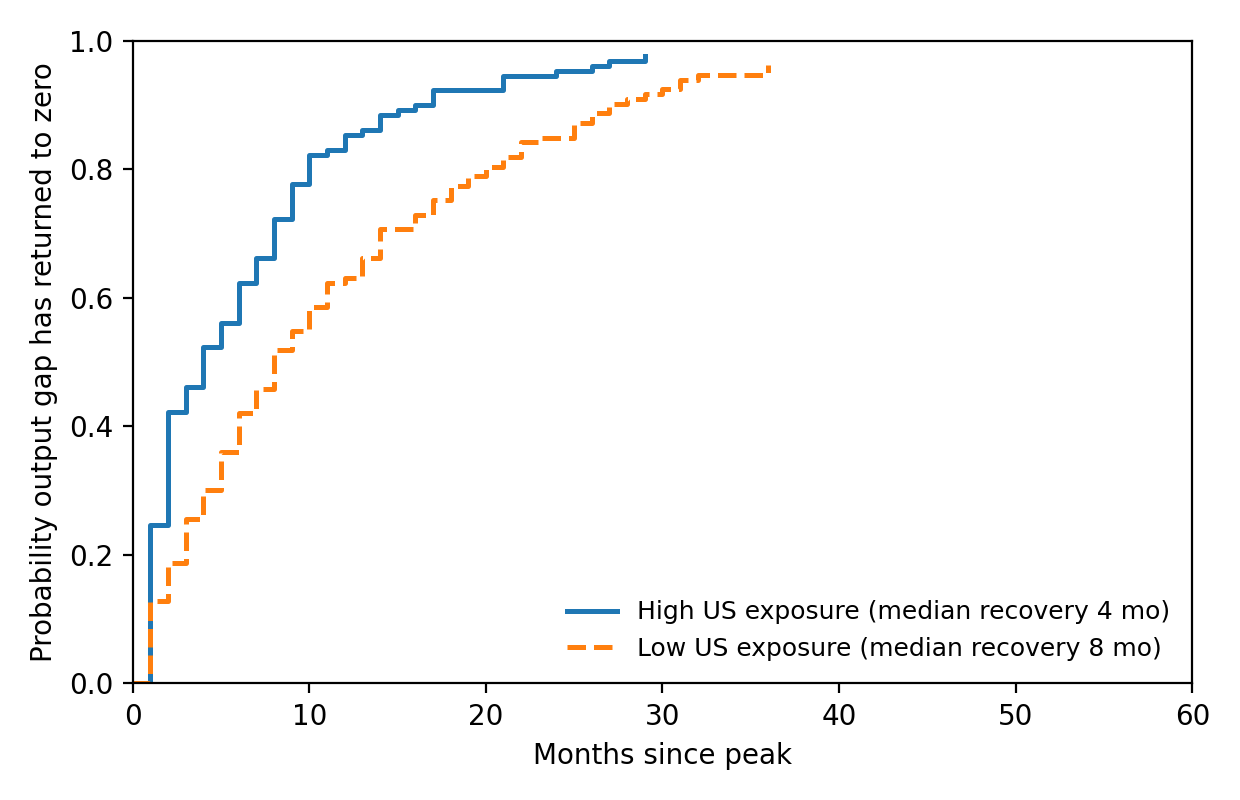
\includegraphics[width=0.78\textwidth]{../output/km_recovery.png}
\caption{Kaplan-Meier recovery curves by US-demand exposure. Each curve is the estimated
probability that an episode's output gap has returned to zero by a given month since the peak, for
episodes above and below the median US-demand pull; episodes not returning within 60 months are
right-censored. The high-exposure group recovers faster at every horizon (median recovery four
months against eight; log-rank $p<0.001$).}
\label{fig:km}
\end{figure}

Figure~\ref{fig:statedep} asks whether the single US-demand coefficient conceals a response that
varies with the depth of the downturn or the size of the pull. The left panel replaces the constant
slope with a smooth functional coefficient, interacting the US-demand pull with a quadratic in the
episode's depth, and traces the implied effect across the observed depth range with a
country-clustered band. The estimated function is close to flat and stays near the linear value at
every depth, and the joint test that it varies with depth does not reject a constant slope.\footnote{The
linear effect is $-5.6$ months ($t=-3.6$); the functional coefficient runs from about $-5.1$ months
at the twenty-fifth percentile of depth to $-4.7$ at the seventy-fifth, and the Wald test of a flat
slope gives $\chi^2(2)=1.02$, $p=0.60$.} The middle panel splits the sample into deep and shallow
downturns at a threshold and reports the difference between the two regime slopes as the threshold
slides from the twenty-fifth to the eightieth percentile of depth. The gap wanders between roughly
$-4$ and $-1$ months and is never significant, so a regime split would report a state-dependence that
is an artifact of where the cut is placed. The right panel repeats the smooth check against the size
of the pull rather than the state, letting the marginal effect vary with the magnitude of the
US-demand pull itself. The point estimates decline in magnitude toward the largest pulls, but the
band contains the linear line throughout and the curvature is not significant, so the data are
consistent with a constant marginal effect while leaving a suggestion of diminishing returns.\footnote{Wald
test of a linear-in-size effect $\chi^2(1)=1.69$, $p=0.19$.} Depth is partly an outcome of the same
recovery process, so these are descriptive interaction checks rather than causal statements about
state, and they support reporting the effect as a single linear coefficient.

\begin{figure}[H]
\centering
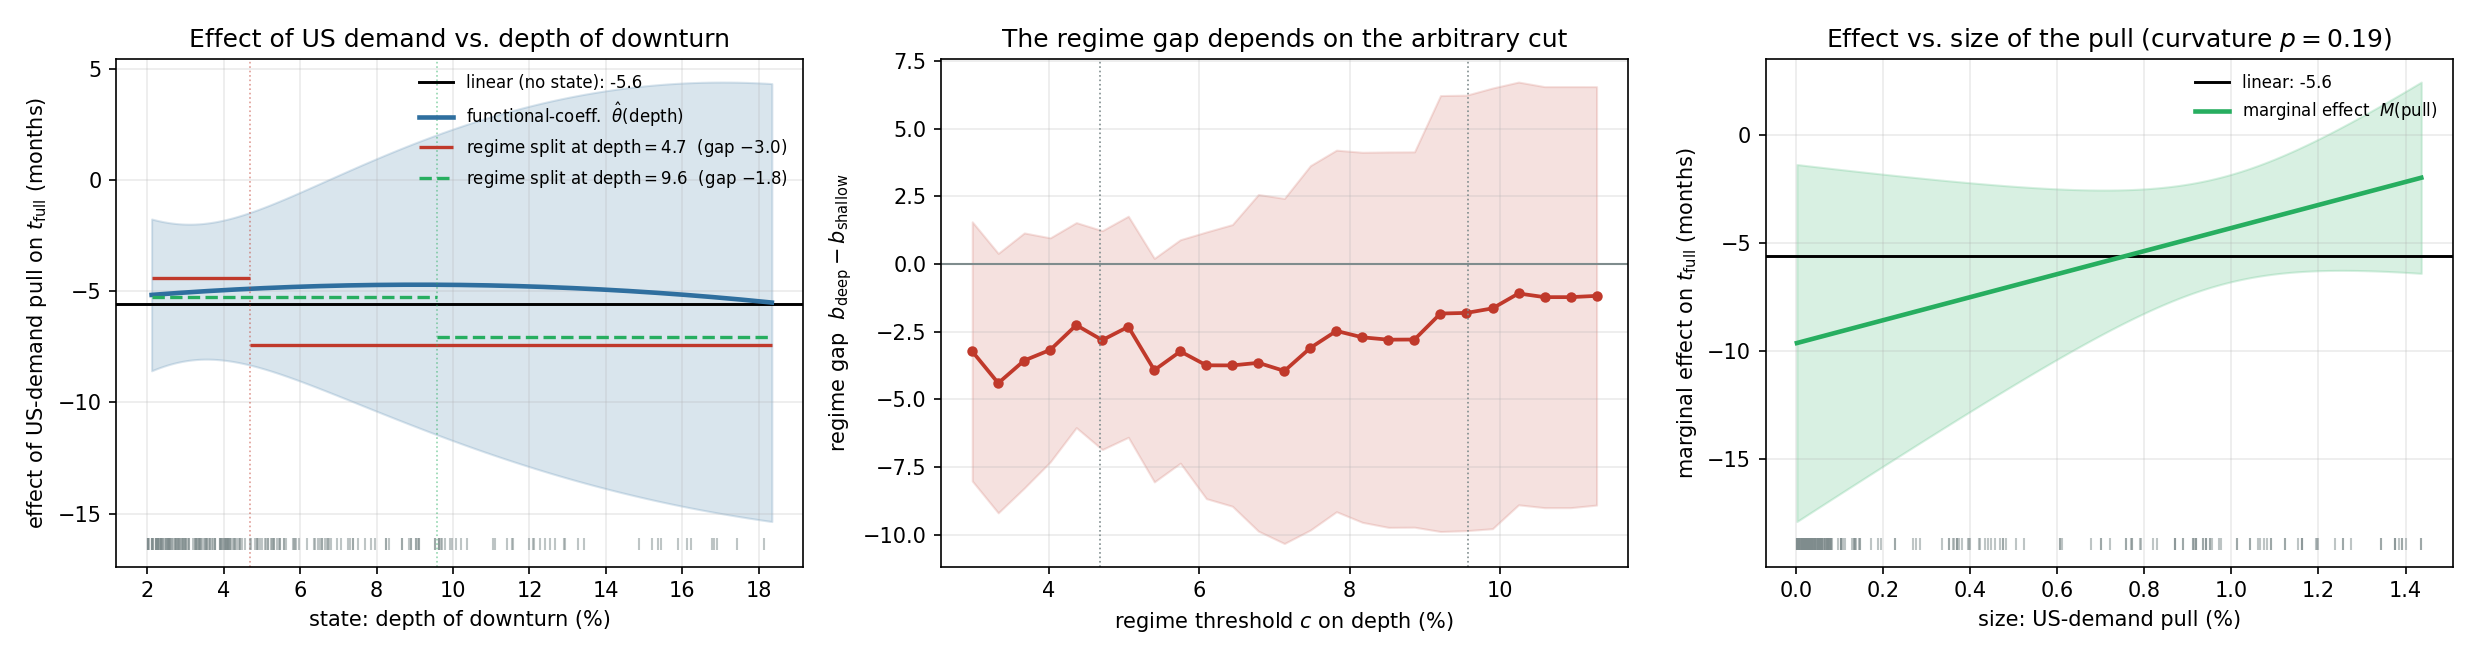
\includegraphics[width=\textwidth]{../output/sdlp_trade_compare.png}
\caption{The US-demand association does not vary with the state or the size of the pull. Left: the effect
of the US-demand pull on full-cycle recovery estimated as a smooth function of the depth of the
downturn (functional coefficient, quadratic interaction), with the flat linear estimate and two
deep-versus-shallow regime splits shown for comparison; the shaded band is a $95\%$ cluster-robust
interval and the ticks mark the depth of each episode. Centre: the difference between the deep and
shallow regime slopes as the regime threshold slides across the depth distribution, showing that the
apparent state-dependence depends on the arbitrary cut. Right: the marginal effect estimated as a
smooth function of the size of the US-demand pull, against the constant linear effect. Standard errors
are clustered by country throughout.}
\label{fig:statedep}
\end{figure}

\section{The dynamic core-periphery model}\label{app:model}

The static portfolio framework clarifies why exposure to a relatively stable external buyer can diversify idiosyncratic demand risk. This appendix presents a small dynamic model to isolate a related mechanism: two expansions of equal size in the core economy can have different effects abroad when their import content differs. The model is deliberately stylized. It is not intended as a quantitative structural model of the United States or as an account of optimal monetary policy. Its purpose is to trace the sequence from the composition of core growth to core import demand, bilateral exports, and the duration of a downturn in a peripheral economy.

\paragraph{The core economy.}
Core activity has two components. The first, $\hat c_t$, is import-intensive absorption, such as household consumption and other expenditure with a relatively high imported content. The second, $\hat q_t$, is import-light domestic activity, such as domestically produced services or production that substitutes for imports. Import-light activity follows an autoregressive process,
\begin{equation}
    \hat q_t = \rho_q \hat q_{t-1} + \varepsilon_t^q,
    \qquad 0<\rho_q<1.
    \label{eq:q_process}
\end{equation}

Import-intensive absorption is forward-looking and can be crowded out by the expansion of the import-light sector,
\begin{equation}
    \hat c_t
    = \mathbb{E}_t \hat c_{t+1}
    - \sigma \hat r_t
    - \chi \hat q_t
    + \varepsilon_t^c,
    \qquad \sigma>0,\quad \chi\geq0.
    \label{eq:core_absorption}
\end{equation}
The term $-\chi\hat q_t$ summarizes competition for labor, capital, and expenditure between the two components. It allows an import-light expansion to displace some import-intensive absorption, without requiring such displacement by assumption.

A small stabilization rule closes the core block,
\begin{equation}
    \hat r_t = \phi_y \hat y_t^{C},
    \qquad \phi_y\geq0.
    \label{eq:small_rule}
\end{equation}
Here $\hat r_t$ is a reduced-form real financing or stabilization rate rather than a fully specified monetary-policy instrument. The rule dampens core activity but is not the source of the model's cross-border result.

Core output combines the two components,
\begin{equation}
    \hat y_t^{C}
    = \omega_c \hat c_t + \omega_q \hat q_t,
    \qquad \omega_c>0,\quad \omega_q>0.
    \label{eq:core_output_new}
\end{equation}
Core imports depend on the import content of each component,
\begin{equation}
    \hat m_t
    = \eta_c \hat c_t + \eta_q \hat q_t,
    \qquad \eta_c>\eta_q\geq0.
    \label{eq:core_imports_new}
\end{equation}
The restriction $\eta_c>\eta_q$ is the central economic assumption: import-intensive absorption generates more foreign demand per unit of activity than import-light production. Combining equations~\eqref{eq:core_absorption} and \eqref{eq:core_imports_new}, the total effect of an import-light expansion on imports contains a positive direct component, $\eta_q$, and a negative displacement component operating through $\hat c_t$. Core imports can therefore rise weakly, remain unchanged, or fall even while core output rises. The result depends on composition rather than on a direct assumption that import-light activity must reduce imports.

\paragraph{Bilateral transmission to the periphery.}
A peripheral economy $i$ receives only the portion of core import demand associated with its predetermined bilateral exposure,
\begin{equation}
    \hat x_{i,t} = \gamma_i \hat m_t,
    \qquad \gamma_i\geq0,
    \label{eq:bilateral_exports}
\end{equation}
where $\gamma_i$ maps the core's aggregate imports into demand for economy $i$'s exports. This parameter is the model counterpart of the pre-downturn bilateral export exposure used in the empirical shift-share measure.

Peripheral activity evolves according to
\begin{equation}
    \hat y_{i,t}^{P}
    = \rho_P \hat y_{i,t-1}^{P}
    + \alpha \hat x_{i,t}
    + \varepsilon_{i,t}^{P},
    \qquad 0<\rho_P<1,\quad \alpha>0.
    \label{eq:periphery_output_new}
\end{equation}
A negative realization of $\varepsilon_{i,t}^{P}$ generates an idiosyncratic downturn. External demand affects the subsequent path through exports, and the strength of the transmission increases with bilateral exposure $\gamma_i$. Unlike the previous specification, the model does not impose an additional buffering-loss multiplier on the domestic shock. Any difference in recovery arises through realized foreign demand.

\paragraph{Equal-output experiments.}
To isolate composition, the import-intensive and import-light shocks are normalized to generate the same impact increase in core output,
\begin{equation}
    \Delta \hat y_0^{C}\big|_{\varepsilon^c}
    =
    \Delta \hat y_0^{C}\big|_{\varepsilon^q}.
    \label{eq:equal_output_normalization}
\end{equation}
Under this normalization, different responses abroad cannot be attributed to a larger core expansion. They arise because the two expansions generate different paths for core imports. Since $\eta_c>\eta_q$, an import-intensive expansion produces a larger import response unless the endogenous adjustment of absorption overturns this ranking.

For each peripheral economy, define recovery as the first period in which activity returns to trend after the domestic downturn,
\begin{equation}
    T_i
    = \min\left\{h\geq0:\hat y_{i,h}^{P}\geq0\right\}.
    \label{eq:recovery_time}
\end{equation}
The model therefore produces a duration outcome comparable to the empirical full negative cycle. Starting from the same negative domestic shock, recovery is faster when the core expansion generates stronger import demand. The difference between the two recovery paths is larger for economies with greater exposure $\gamma_i$.

\begin{proposition}[Composition of core growth and peripheral recovery]
\label{prop:composition_recovery}
Consider two shocks that generate the same impact increase in core output. If the import-intensive shock generates a larger path of core imports than the import-light shock, then for any peripheral economy with $\alpha\gamma_i>0$,
\[
    \hat y_{i,t}^{P,c} \geq \hat y_{i,t}^{P,q}
\]
for every horizon at which the cumulative import-demand difference is nonnegative. If the inequality is strict before either path returns to trend, then
\[
    T_i^{c} \leq T_i^{q}.
\]
The difference between the two activity paths is increasing in bilateral exposure $\gamma_i$.
\end{proposition}

\begin{proof}
Subtract equation~\eqref{eq:periphery_output_new} under the two core shocks. With the same domestic shock and initial condition,
\[
    \Delta \hat y_{i,t}^{P}
    = \rho_P \Delta \hat y_{i,t-1}^{P}
    + \alpha\gamma_i\Delta \hat m_t,
\]
where $\Delta \hat m_t=\hat m_t^{c}-\hat m_t^{q}$. Iterating forward gives
\[
    \Delta \hat y_{i,t}^{P}
    = \alpha\gamma_i
      \sum_{j=0}^{t}\rho_P^{t-j}\Delta \hat m_j.
\]
Because $\alpha\geq0$, $\gamma_i\geq0$, and $\rho_P\geq0$, a nonnegative discounted cumulative import-demand difference implies a nonnegative difference in peripheral activity. A strictly higher activity path before recovery cannot cross zero later than the lower path. The expression is linear in $\gamma_i$, establishing that the difference is larger for more exposed economies.
\end{proof}

\paragraph{Interpretation.}
The small stabilization rule in equation~\eqref{eq:small_rule} affects the magnitude and persistence of both core expansions by moderating import-intensive absorption. It does not create the model's central ranking, which follows from the difference in import content and the bilateral exposure channel. Setting $\phi_y=0$ removes the stabilization response; increasing $\phi_y$ dampens the propagation of both shocks. The qualitative comparison survives whenever the import-intensive expansion continues to generate the larger discounted path of core imports.

The model separates three cases. First, when import-light activity has positive but low import content and only weakly displaces absorption, core imports rise, but by less than under an equal-sized import-intensive expansion. Second, when its direct import content approximately offsets the displaced absorption, core output rises with little change in imports. Third, when displacement dominates, as may occur under import substitution or reshoring, core output rises while imports fall. In all three cases, the external support received by the periphery depends on the composition of core growth and on the economy's predetermined exposure to the core market.

\paragraph{Calibration and simulation.}
The model is calibrated to illustrate the mechanism rather than to match all features of the US and
peripheral economies, so the responses are qualitative. Table~\ref{tab:calib} lists the values. The
import-content parameters satisfy $\eta_c>\eta_q$, the central assumption; the displacement
parameter $\chi$ is small, so an import-light expansion still raises core output; and the bilateral
exposure $\gamma_i$ takes a low and a high value spanning the range of pre-downturn US export
exposure in the data. The linearized system is solved by backward recursion of the forward-looking
absorption equation, and each core expansion is a persistent ($\rho=0.7$) push normalized to the
same impact rise in core output.

\begin{table}[H]
\centering\small
\caption{Calibration of the dynamic illustration (quarterly).}
\label{tab:calib}
{\setlength{\tabcolsep}{5pt}
\begin{tabular}{@{}lll@{\hskip 1.5em}lll@{}}
\toprule
Parameter & Meaning & Value & Parameter & Meaning & Value \\ \midrule
$\rho_q$ & import-light persistence & 0.70 & $\omega_c,\omega_q$ & output shares & 0.55, 0.45 \\
$\sigma$ & intertemporal elasticity & 1.00 & $\eta_c$ & import content, intensive & 0.60 \\
$\chi$ & displacement of absorption & 0.05 & $\eta_q$ & import content, light & 0.25 \\
$\phi_y$ & stabilization rule & 0.15 & $\rho_P$ & periphery persistence & 0.70 \\
$\alpha$ & export pass-through & 0.80 & $\gamma_i$ & bilateral exposure (low/high) & 0.10 / 0.35 \\
\bottomrule
\end{tabular}}
\end{table}

Figure~\ref{fig:layer2} reports the result. Normalized to the same impact rise in core output
(left panel), the import-intensive expansion generates a much larger path of core imports than the
import-light one (centre: about $1.1$ against $0.2$ on impact, and roughly $3.6$ against $0.8$
cumulated over the horizon shown). Starting from the same domestic downturn, a peripheral economy
exposed to the import-intensive expansion returns to trend faster the higher its bilateral exposure
(right: about three quarters at $\gamma=0.35$ against eleven at $\gamma=0.10$). The figure maps the
model directly to the paper's empirical result: a growing hub supports recovery only to the extent
that its growth translates into demand for the peripheral economy's exports.

\section{Data and code}\label{app:code}
The bilateral trade data are from the IMF's International Trade in Goods Statistics (IMTS) and the
GDP data from the IMF World Economic Outlook, both accessible through the IMF's data portal; the
intensity variables used in the services robustness are from the World Bank's World Development
Indicators (WDI). The monthly activity indicators are drawn from Haver Analytics under a commercial
license and cannot be redistributed, but the series identifiers and construction are documented in
the replication code. The dynamic core-periphery illustration is solved as a linearized system and
simulated with the author's own Python code (\texttt{scripts/model\_dynamic.py} in the replication
package). The leave-one-out import-demand shift, its exposure-robust standard errors, and the
validation battery of Appendix~\ref{app:robust} are built by
\texttt{scripts/identification\_loo.py}. The estimation and figure code, and the pull scripts for
the public data, are available from the author on request.


% ============================================================================
%  IMF BACK COVER PAGE
% ============================================================================
\definecolor{imfblue}{RGB}{0,72,144}
\clearpage
\thispagestyle{empty}
\null
\begin{tikzpicture}[remember picture, overlay]
    % Full-page IMF blue background (no spine strip)
    \fill[imfblue] (current page.south west) rectangle (current page.north east);
    % Real IMF seal (white), sitting just above the title block
    \node[anchor=south west, inner sep=0pt]
        (seal) at ([xshift=2cm, yshift=7.6cm]current page.south west)
        {
\includegraphics[width=2.1cm]{../imf_seal_white.png}};
    % Vertical rule between seal and text
    \draw[white, line width=1.2pt]
        ([xshift=0.45cm, yshift=-0.55cm]seal.east) --
        ([xshift=0.45cm, yshift=0.55cm]seal.east);
    % PUBLICATIONS wordmark next to the seal
    \node[anchor=west, text=white, font=\sffamily\bfseries\LARGE]
        at ([xshift=0.75cm]seal.east)
        {PUBLICATIONS};
    % Title and WP number, lower-left (regular weight, matching published WP)
    \node[anchor=south west, text=white, font=\sffamily\normalsize, align=left,
          text width=0.60\paperwidth]
        at ([xshift=2cm, yshift=5.0cm]current page.south west)
        {\PaperTitle};
    \node[anchor=south west, text=white, font=\sffamily\normalsize]
        at ([xshift=2cm, yshift=4.2cm]current page.south west)
        {Working Paper No.\ WP/26/XX};
\end{tikzpicture}

\end{document}
